\documentclass[10pt,a4paper,oneside]{scrartcl}

% packages
\usepackage{scrhack}
\usepackage{fullpage}
\usepackage{graphicx}
\usepackage[style=numeric,backend=bibtex8,urldate=iso8601]{biblatex}
\usepackage{listings}
\usepackage{courier}
\usepackage{array}
\usepackage{tabularx}
\usepackage{amsmath}
\usepackage{longtable}
\usepackage[iso]{datetime}
\usepackage{pdfpages}
\usepackage[utf8]{inputenc}

% basic latex configuration
\setlength{\parskip}{\baselineskip}
\setlength{\parindent}{0pt}

% biblatex
\addbibresource{references.bib}

% graphics
\graphicspath{ {./images/} {../latex/images/} } % also import images from theoretical thesis

% language listings
\lstdefinelanguage{CL}[ANSI]{C}
{
	morekeywords={__kernel,kernel,__local,local,__global,global,__constant,constant,__private,private},
	morekeywords={char2,char3,char4,char8,char16,uchar,uchar2,uchar3,uchar4,uchar8,uchar16,short2,short3,short4,short8,short16,ushort,ushort2,ushort3,ushort4,ushort8,ushort16,int2,int3,int4,int8,int16,uint,uint2,uint3,uint4,uint8,uint16,long2,long3,long4,long8,long16,ulong,ulong2,ulong3,ulong4,ulong8,ulong16,float2,float3,float4,float8,float16,image2d_t,image3d_t,sampler_t,event_t,bool,bool2,bool3,bool4,bool8,bool16,half2,half3,half4,half8,half16,quad,quad2,quad3,quad4,quad8,quad16,complex,imaginary},
	morekeywords={convert_char2,convert_char4,convert_char8,convert_char16,convert_uchar,convert_uchar2,convert_uchar4,convert_uchar8,convert_uchar16,convert_short,convert_short2,convert_short4,convert_short8,convert_short16,convert_ushort,convert_ushort2,convert_ushort4,convert_ushort8,convert_ushort16,convert_int,convert_int2,convert_int4,convert_int8,convert_int16,convert_uint,convert_uint2,convert_uint4,convert_uint8,convert_uint16,convert_long,convert_long2,convert_long4,convert_long8,convert_long16,convert_ulong,convert_ulong2,convert_ulong4,convert_ulong8,convert_ulong16,convert_float,convert_float2,convert_float4,convert_float8,convert_float16}
	morekeywords={write_imagef,write_imagei,write_imageui,read_imagef,read_imagei,read_imageh,read_imageui,get_image_width,get_image_height,get_image_depth,get_image_channel_data_type,get_image_channel_order,get_image_dim,get_work_dim,get_global_size,get_global_id,get_local_size,get_local_id,get_num_groups,get_group_id,cross,dot,distance,length,normalize,fast_distance,fast_normalize,isequal,isnotequal,isgreater,isgreat,erequal,isless,islessequal,islessgreater,isfinite,isinf,isnan,isnormal,isordered,isunordered,signbit,any,bitselect,select,async_work_group_copy,wait_group_events,prefetch,barrier,mem_fence,read_mem_fence,write_mem_fence,acos,acosh,acospi,asin,asinh,asinpi,atan,atan2,atanh,atanpi,atan2pi,cbrt,ceil,copysign,cos,cosh,cospi,erfc,erf,exp,exp2,exp10,expm1,fabs,fdim,floor,fma,fmax,fmin,fmod,fract,floor,frexp,hypot,ilogb,ldexp,lgamma,lgamma_r,log,log2,log10,log1p,logb,mad,modf,nan,nextafter,pow,pown,powr,remainder,remquo,rint,rootn,round,rsqrt,sin,sincos,sinh,sinpi,sqrt,tan,tanh,tanpi,tgamma,trunc,half_cos,half_divide,half_exp,half_exp2,half_exp10,half_log,half_log2,half_log10,half_powr,half_recip,half_rsqrt,half_sin,half_sqrt,half_tan,native_cos,native_divide,native_exp,native_exp2,native_exp10,native_log,native_log2,native_log10,native_powr,native_recip,native_rsqrt,native_sin,native_sqrt,native_tan,mad24,mul24,mul_hi,sub_sat,rotate,mad_sat,clz,rhadd,hadd,add_sat,abs_diff,abs,max,min,upsample,get_global_offset,minmag,maxmag,clamp,async_work_group_strided_copy,vec_step,shuffle,shuffle2}
	sensitive=true,
	morecomment=[l]{//},
	morecomment=[s]{/*}{*/},
	morestring=[b]",
}

\lstset
{
	tabsize=2,
	captionpos=b,
	basicstyle=\ttfamily{},
	aboveskip=\parskip,
% keywordstyle=\color{blue}\bfseries,
% commentstyle=\color{commentgreen},
% stringstyle=\color{red},
	showstringspaces=false,
	breaklines=true,
	numbers=left,
	frame=single,
% backgroundcolor=\color{lightgray}
}

\title{GPGPU accelerated visualization of complex geometries}
%\subtitle{}
\author{Bernhard Manfred Gruber}
\date{\today}

\begin{document}

\includepdf{titlepage}
%\maketitle
%\thispagestyle{empty}
%\clearpage

\pagenumbering{Roman}


Declaration

 

I hereby declare and confirm that this thesis is entirely the result of my own original work. Where other sources of information have been used, they have been indicated as such and properly acknowledged. I further declare that this or similar work has not been submitted for credit elsewhere.

%\section*{Acknowledgments}

I want to thank my professor Herwig Mayr for putting in a good work for me at the RISC software company GmbH. On the technical site, I also want to thank my supervisor at RISC, Alexander Leutgeb, for the excellent support on all subjects of the project. Personally, also a thank you for several interesting discussions we have held after work. Furthermore, I want to give thanks to the RISC company itself, for providing me with high quality equipment and an amazing work station during my three month internship which made working a pleasure. Finally, also a thumb-up to Michael Hava for having the most in-depth C++ knowledge of a human being I have ever met. I learned a great deal by reading your code.


\section*{Abstract}

This thesis provides a quick introduction into programming for GPUs using OpenCL. After a historical overview of how graphic cards have evolved, the peculiarities of GPU and CPU hardware are discussed. Based on this knowledge OpenCL is introduced as an API supporting all kinds of processing hardware. A deep look into OpenCL's execution and memory model, which allows handling heterogeneous hardware, is rounded off by a simple, yet full example code.

The thesis then continues with several implementations of standard algorithms for the GPU. The chosen problems start with matrix multiplication and go along with the all-prefix sum and sorting. As the first problem already offers parallelism naturally, performance analysis and optimization is focused during the first implementation chapter. The all-prefix sum and sorting are both problems being more difficult to be split into independent pieces of work. Techniques will be discussed to tackle such kind of problems.

Each GPU implementation is benchmarked and compared with one or more traditional CPU approaches. As GPUs and CPUs feature different hardware architectures, appropriate algorithms and optimizations have been chosen to solve the problems by exploiting the underlying platform at best.


\tableofcontents

\clearpage

\pagenumbering{arabic}

\section{Introduction}


\subsection{Motivation}
why is this goal important?
what could be improved? (how far?)
how could make use of this? (which companies, domains, areas of application, all?)

\subsection{Goal}
what does this document show?
GPGPU acceleration with OpenCL
what is OpenCL? what is GPGPU computing?
example implementations of matrix multiplication, prefix sum and sorting alg.

what is the outcome of my work? (which algorithms profit from GPGPU acc, acceleration vs. invested time)


how do I get to this outcome? (chosen algorithms, used implementations, reference implementations, benchmarks)

\subsection{Chapter overview}




\section{Fundamental principles}

\subsection{Raycasting}

\subsection{Acceleration structures}

\subsection{Boolean raycasting}


\section{Existing prototype}


\subsection{Structure}
class diagram

organisation

vs solution


\subsection{Data structure}

regular grid

macro/micro cells

triangles in cells, pointer to sweep volumes


\subsection{Classification}

description of classification algorithm (principle)

images from RISC presentation

\begin{figure}
\centering
\includegraphics[width=0.4\linewidth]{classification}
\caption{Principle of classifying cells of the grid.}
\label{fig:classification}
\end{figure}

\begin{figure}
\centering
\includegraphics[width=0.4\linewidth]{classification_sub}
\caption{Classification result after adding a subtraction volume. }
\label{fig:classification_sub}
\end{figure}

\subsection{Adapted raycasting algorithm}

consequences of classification on raycasting algorithm

implicit geometry, water tightness? why no problem?

algorithm description of CPU caster


\section{OpenCL ray casters}
\label{sec:opencl_caster}

Before altering the existing prototype after its analysis, a separate branch in SVN has been created to allow experimenting with the existing code without disturbing the other members of the team. Before development could be started, further tools had to be installed. As the GPU provided by RISC was from NVIDIA, NVIDIA's CUDA Toolkit (version 5.0) was installed which contains the required OpenCL header files and libraries. Furthermore, the OpenCL C++ wrapper provided by Khronos (cl.hpp) was downloaded from their website. Several weeks later, also Intel's SDK for OpenCL Applications 2013 was added, which provided a limited OpenCL debugger some smaller extensions to Visual Studio. Then, a separate project was added to the existing Visual Studio solution and the necessary include and library paths configured in order to use OpenCL.

\subsection{OpenCL ray casting driver}

Implementing a ray caster with OpenCL started by designing a small infrastructure which should fulfill some requirements:

\begin{itemize}
	\item Only one class should be needed by \lstinline!DebugView! (the main application class) in order to communicate with the OpenCL ray caster.
	\item As the OpenCL ray casters will be developed incrementally and several different ideas exists, it should be possible to write multiple, interchangeable casters.
	\item It should be possible to reload an OpenCL caster at run time. As loading larger scenes may take up to some minutes and the OpenCL source code is read in and compiled at run time, this feature allows it to change the OpenCL source code of a caster at run time and reload it without having to relaunch the host application.
	\item Several options should be adjustable by the main application via the console (which may trigger a recompilation of the kernels or a reconfiguration of the OpenCL environment).
	\item If a ray caster crashes or OpenCL experiences any problems, it should be possible to relaunch the complete OpenCL environment without having to restart the whole application. 
\end{itemize}

Derived from these requirements, a simple architecture has been designed which is shown in the simplified class diagram in figure \ref{fig:enlight_opencl_class_diagram}.

\begin{figure}
\centering
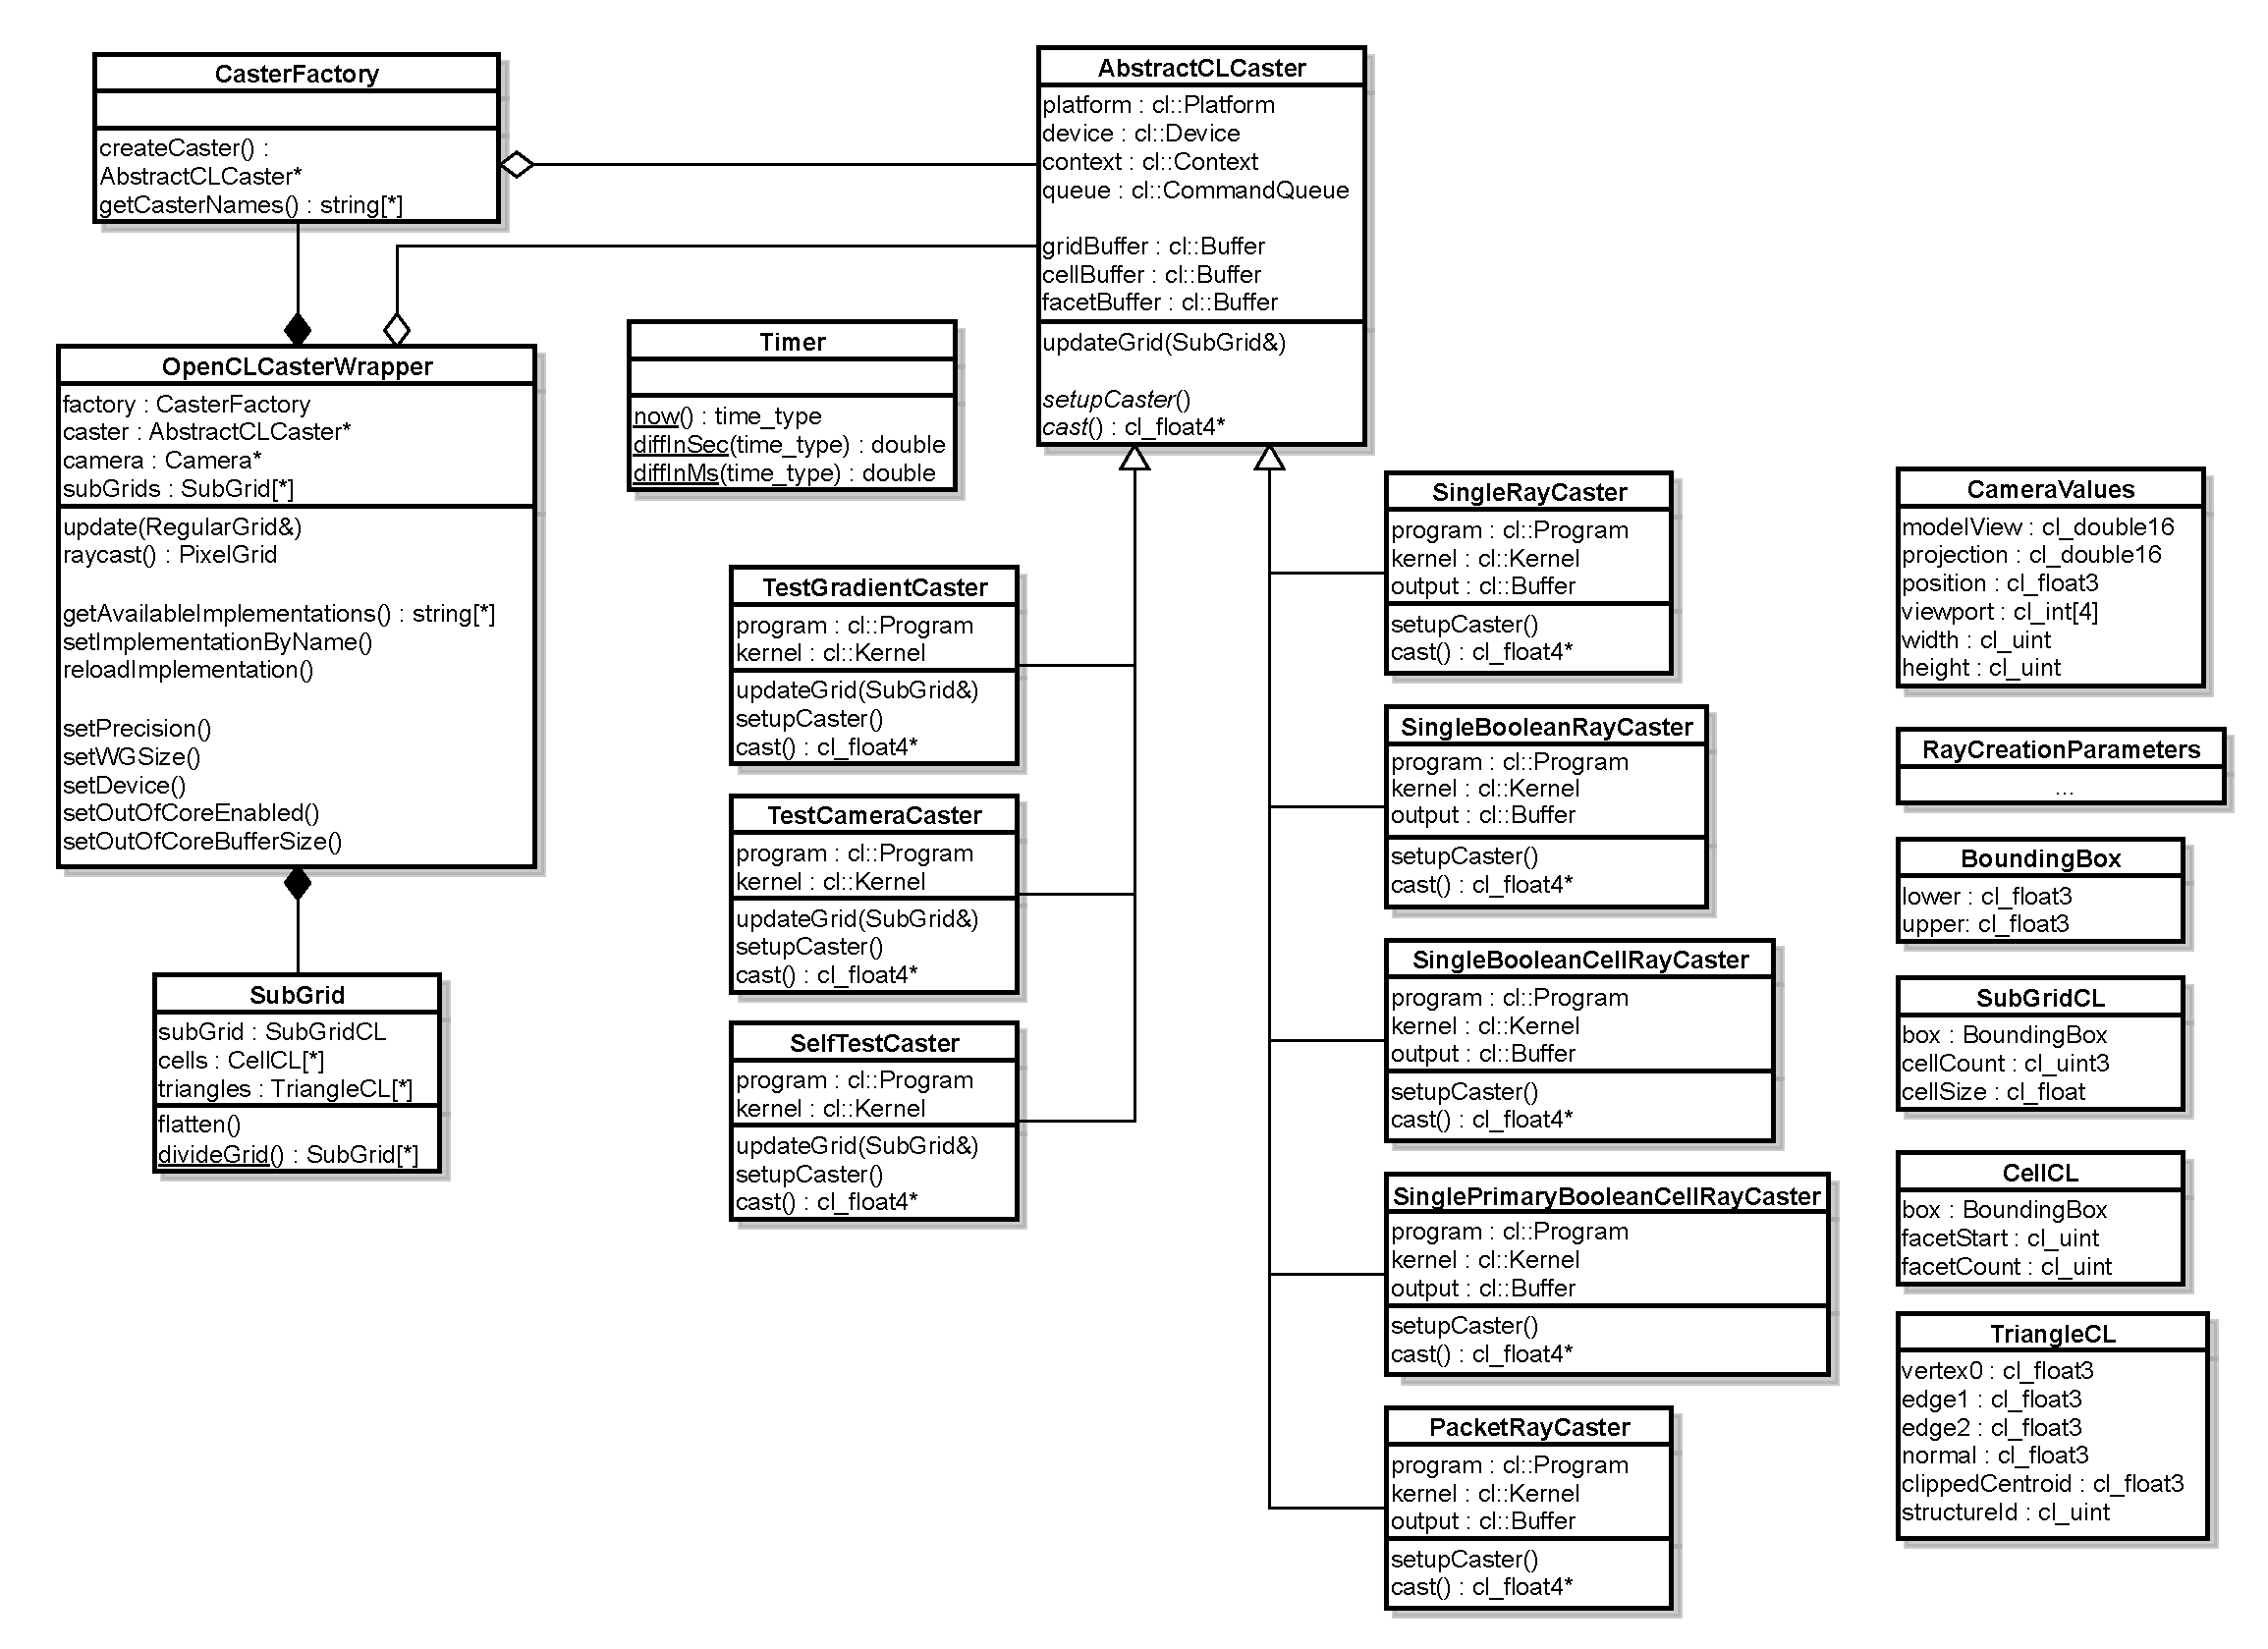
\includegraphics[width=\textwidth]{enlight_opencl_class_diagram}
\caption{Simplified class diagram of the OpenCL ray casting driver.}
\label{fig:enlight_opencl_class_diagram}
\end{figure}

The central class and entry point of the OpenCL ray casting environment is the \lstinline!OpenCLCasterWrapper! class. An instance of this class is maintained by \lstinline!DebugView!, similar to the \lstinline!RayCasterWrapper! (cf. figure \ref{fig:enlight_class_diagram}). The \lstinline!OpenCLCasterWrapper! offers several methods for interacting with an OpenCL caster. Most importantly, it offers an \lstinline!update! method taking a reference to the \lstinline!RegularGrid! maintained by the main application which holds all relevant data of the scene. This method has to be called at least once before ray casting can be done. The \lstinline!raycast! method performs the main work of generating an image. The created image with depth information is also stored inside an object of \lstinline!PixelGrid! and passed back to the main application. \\
For managing the underlying ray casting implementations, each caster is assigned a name. This assignment is managed by the \lstinline!CasterFactory!, which is used by the \lstinline!OpenCLCasterWrapper! to provide a list of available implementations and to allow selection and creation of casters by their name. The currently loaded caster is pointed to by the \lstinline!caster! member of the \lstinline!OpenCLCasterWrapper!. Furthermore, a reload method is provided for recreating the currently loaded caster. \\
Additionally, several options concerning OpenCL and the implemented ray casters may be set by the main application using the console. The \lstinline!OpenCLCasterWrapper! offers further methods for configuring several values such as the used floating point precision, work group size, OpenCL platform and device as well as enabling out of core casting and adjusting the out of core buffer size (cf. chapter \ref{sec:out_of_core}).

The \lstinline!SubGrid! class is responsible for holding the full or a part of the grid. and for transforming the grid's representation into buffers which can be pushed to the GPU. Details to both usages will be discussed with the caster implementations requiring this functionality.

The \lstinline!Timer! class is a small helper class for measuring durations. It is used to print to the time required for certain operations inside the driver such as ray casting a frame, compiling a kernel or ray casting an out of core mesh in multiple passes.

The second most important class is \lstinline!AbstractCLCaster!. It is the base of all ray caster classes and is responsible for setting up the OpenCL environment for each caster. Every ray caster implementation has to inherit from this class and must implement the both pure virtual functions \lstinline!setupCaster! and \lstinline!cast!. While \lstinline!cast! is called directly from the \lstinline!OpenCLCasterWrapper!, \lstinline!setupCaster! is a template method inside \lstinline!AbstractCLCaster! and is called during the casters construction, after OpenCL has been initialized. The derived caster implementation should create its kernels and further resources here. The \lstinline!updateGrid! method is already implemented in the base class, as it works equally for all ray casting implementations which require the grid on the GPU (all non-test casters). Furthermore, \lstinline!AbstractCLCaster! offers a variety of utility methods which can be used by derived casters.

On the right side of the class diagram (figure \ref{fig:enlight_opencl_class_diagram}) are several structures. \lstinline!CameraValues! is used to transport relevant camera information from the \lstinline!OpenCLCasterWrapper! into the caster implementations. This avoids dragging the \lstinline!Camera! class and its dependencies deeper into the OpenCL project (The grid is also converted into one or multiple instances of \lstinline!SubGrid! before it is passed into the caster implementations in order to reduce avoidable dependencies). The remaining structures are all used as data transfer objects between the OpenCL ray casters on the host application and the GPU. Therefore, only types defined in the corresponding OpenCL header are used (e.g. \lstinline!cl_uint!, \lstinline!cl_float3!). 


\subsection{TestGradientCaster}

The first caster is a proof of concept to test the functionality of the OpenCL environment. It does not use the grid, loaded geometries or the camera's current values. The \lstinline!TestGradientCaster! only loads the OpenCL kernel source code from a file and compiles it using corresponding helper methods from \lstinline!AbstractCLCaster! inside the overridden \lstinline!setupCaster! method. The \lstinline!updateGrid! method is also overridden but empty, as no grid buffers have to be created and uploaded. Inside the \lstinline!cast! method, an output buffer is created capable of holding a \lstinline!cl_float4! value (red, green, blue, depth) for each pixel of the requested output image (determined by the fields \lstinline!width! and \lstinline!height! of \lstinline!CameraValues!, of which an instance is passed to the \lstinline!cast! method). Then, the loaded kernel is enqueued on the command queue for execution on the GPU. The global work size of the kernel is only one dimensional and the number of output pixels rounded up to be a multiple of the maximum allowed work group size. Each kernel invocation then derives the output pixels x and y coordinate from the global id of the work item and writes a color value to the output buffer. The red channel of the color is the x coordinate divided by the output image width, the green channel is the y coordinate divided by the height and the blue and depth channel are set to zero. After the kernel has executed, the result is read back to the host into an allocated \lstinline!cl_float4! array, which is then returned by the \lstinline!cast! method. The \lstinline!OpenCLCasterWrapper! converts this array into an instance of \lstinline!PixelGrid! which is then passed back to the main application for display.

The resulting gradient of the TestGradientCaster is shown in figure \ref{fig:testgradient}.

\begin{figure}[h]
\centering
\includegraphics[width=0.5\textwidth]{testgradient}
\caption{Screenshot of the OpenCL kernel output of the TestGradientCaster.}
\label{fig:testgradient}
\end{figure}


\subsection{TestCameraCaster}

The next test caster is based on the \lstinline!TestGradientCaster!. The goal of this caster is to test the creation of rays according to the current camera settings. Therefore, the \lstinline!CameraValues! instance passed to the \lstinline!cast! method is converted into a \lstinline!RayCreationParameters! structure, which is passed as an argument to the kernel. This structure contains selected fields of the model view and projection matrix as well as several precalculated values which are used to create the ray direction vectors for a given x and y coordinate on the image plane. The kernel itself stores the vertices of 12 triangles forming a simple cube placed at the coordinate space origin in constant memory (a special part of the global memory). The kernel is enqueued with a two dimensional global work size of the output images width and height (both rounded up to be a multiple of the configured work group size). Each work item than calculates the ray direction of the ray traveling through the pixel of the work group item's x and y coordinate on the image plane. With the origin at the camera position, this ray is then intersected with the 12 triangles of the cube. The intersection routine used is an adapted version of the "Fast, Minimum Storage Ray/Triangle Intersection" (name of the paper) approach presented by Tomas Möller and Ben Trumbore. \cite{triangle_intersection}. The intersections are depth sorted to find the correct intersection point and hit triangle. A color value for the pixel is then calculated using the dot product of the ray's direction vector and the surface normal of the hit triangle. After the kernel has run, the resulting buffer is processed as by the TestGradientCaster.

%\subsubsection{Ray creation routines}
%
%ray creation parameters, matrices, formulas

%\subsubsection{Fast triangle intersection routine}
%
%paper + explanation

The resulting image of a cube which rotates synchronously with the OpenGL visualization of the loaded scene is shown in figure \ref{fig:testcamera}.

\begin{figure}[h]
\centering
\includegraphics[width=0.5\textwidth]{testcamera}
\caption{Screenshot of the OpenCL kernel output of the TestCameraCaster.}
\label{fig:testcamera}
\end{figure}


\subsection{SelfTestCaster}

The self test caster is a simple test of the structures used in host application and OpenCL interaction. More specifically, the SelfTestCaster calculates the size of all structures used in memory transfers between the host and the GPU on the host and enqueues a kernel retrieving the corresponding values on the device side. These values are compared against each other and an error is yielded if any pair of them is not equal.
The reason why problems might occur on this level is the varying struct member alignment and padding carried out by different compilers. Although the data alignment of OpenCL is based on the one of ISO C99, some additions have to be made for OpenCL's built in vector types (cf. OpenCL specification 6.1.5 \cite{opencl_spec}). In particular, OpenCL has built in vector types which have to be aligned to a memory address being an even multiple of their size and a power of two. A \lstinline!float3! value for example, with a theoretical size of 12 bytes, is therefore aligned to a 16 byte boundary. However, the corresponding \lstinline!cl_float3! typedef on the host application (defined in cl.h) is backed by a structure containing a four element float array. This ensures that both types, \lstinline!float3! inside OpenCL and \lstinline!cl_float3! on the host application, are of equal size (16 byte), but it cannot guarantee a proper alignment as the OpenCL \lstinline!float3! type will be 16 bytes aligned and the \lstinline!cl_float3! structure (an array of floats) only to a four byte boundary. This has significant consequences if such vector types are used within structures as the size of the structs may be different (typically larger) inside an OpenCL kernel than within the host application. Consequently, enforcing proper alignment is partially up to the programmer and has to be declared for the affected structures (e.g. with \lstinline! __declspec(align(sizeof(cl_float3)))! using Intel's C++ compiler).
As the kernel does not create an output image, an empty buffer is allocated on the host and returned.


\subsection{SingleRayCaster}

The SingleRayCaster is the first full ray casting attempt. It is based on the TestCameraCaster considering the host code, the ray creation inside the work items and the triangle intersection routine. However, instead of using statically coded geometry inside the kernel, the grid containing the loaded geometries from the main application is used. Therefore, an appropriate memory layout has to be defined which fits well to the concept of OpenCL buffers. To traverse the grid, the 3D DDA algorithm presented in chapter \ref{sec:regular_grids} has to be implemented. No counting is performed and no distinction of triangles from different structures and their facing (normal vector) is made.

As the data structure holding the grid on the host application is to some degree hierarchical (grid uses dynamically allocated array of cells, cells hold arrays of pointers to facets), the first step before any transfer to the GPU can happen is to flatten the data structure into corresponding OpenCL buffers. Figure \ref{fig:buffer_layout} shows how the grid data structure can be represented using linear arrays by substituting pointers by indexes.

\begin{figure}[h]
\centering
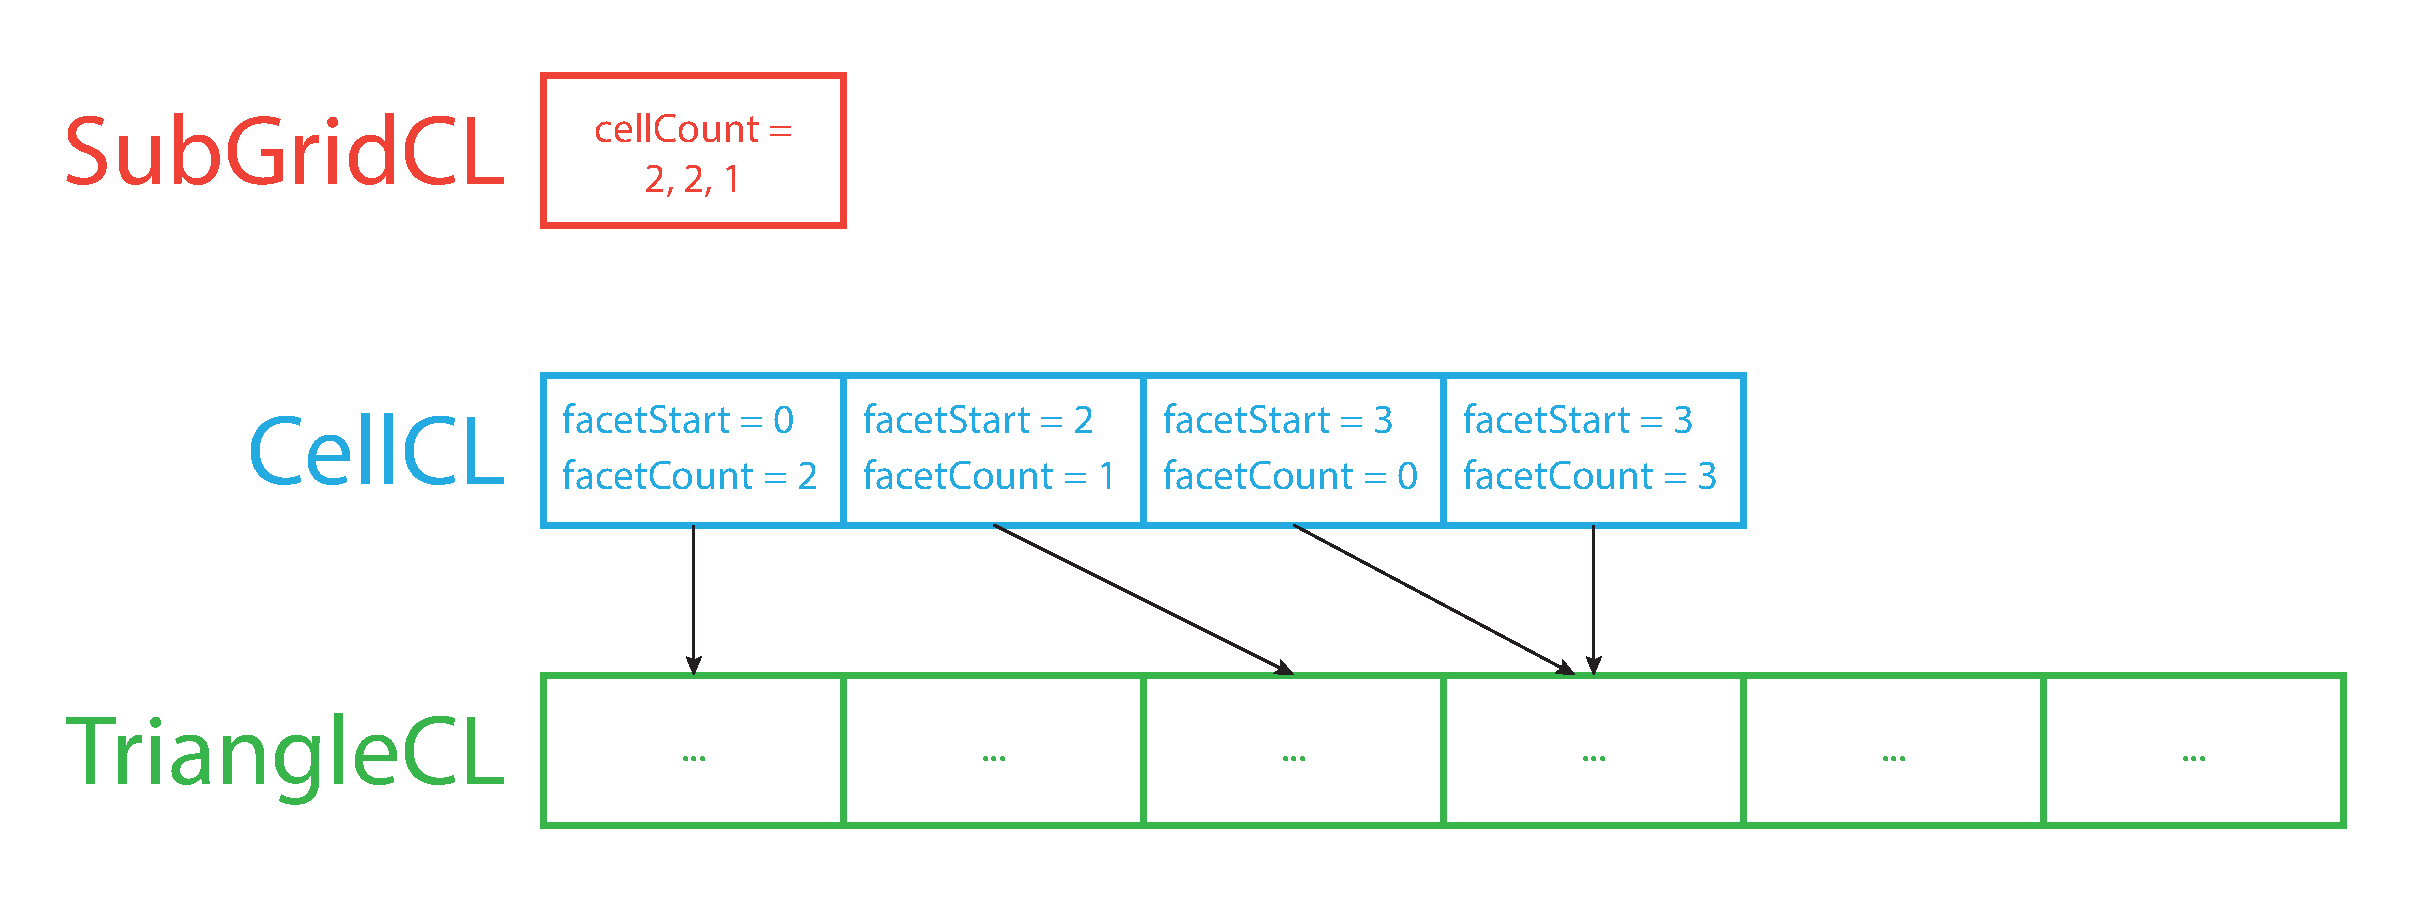
\includegraphics[width=0.8\textwidth]{buffer_layout}
\caption{Layout of the OpenCL buffers used to store the flattened grid.}
\label{fig:buffer_layout}
\end{figure}

Three buffers are required to store the grid. The first on is rather small and only stores meta information about the grid. It contains a single instance of the \lstinline!SubGridCL! struct which contains the \lstinline!cellCount! member. This cell count holds the extents of the grid in all three dimensions and therefore determines the number of cells.
The second buffer stores the cells as a large array of \lstinline!\CellCL! structures. Each of them may have multiple facets associated with them. Therefore, each cell has a \lstinline!facetStart! index which points to the first of \lstinline!facetCount! triangle belonging to this cell in the triangle buffer.
The third buffer then holds a huge array of triangles which contain the geometric information about the scene.

Flattening the grid into these three buffers has to be done every time a surface cell changes (e.g. by loading a new subtraction volume). When an update of the grid has occurred, the main application calls the \lstinline!OpenCLCasterWrapper!s \lstinline!update! method and passes the reference to the new grid. The grid is then flattened by the \lstinline!SubGrid! class, filling its members \lstinline!subGrid!, \lstinline!cells! and \lstinline!triangles!, which are exactly the contents of the three required OpenCL buffers. The \lstinline!SubGrid! instance is then passed to the currently loaded caster by calling the \lstinline!updateGrid! method. This method is implemented in \lstinline!AbstractCLCaster! and creates the actual OpenCL buffer objects and transfers the content of the \lstinline!SubGrid! to the GPU.

The kernel itself is again enqueued with a two-dimensional global work size of the size of the output image (one work item per pixel) rounded up to a multiple of the configured work group size. The kernel code for this first full ray casting approach starts equally as the TestCameraCaster. Each work item initially determines its ray direction. Then, the grid has to be traversed using the adapted 3D DDA algorithm based on John Amanatides and Andrew Woo presented in chapter \ref{sec:regular_grids} \cite{3DDDA}. This algorithm basically works by calculating the entry point of the ray into the grid as well as the corresponding cell of this entry point. Then, increment values for each dimension are calculated which are used to determine the next cell from the current one (details can be found corresponding paper). The collection of routines implementing this algorithm will be called cell traverser. After initialization, the ray casting kernel polls cells from this cell traverser until an intersection has been found or the grid has been fully traversed. For each cell returned by the cell traverser, all triangles inside this cell (determined by the \lstinline!facetStart! and \lstinline!facetCount! members)) are loaded from the triangle buffer and intersected using the same routine as in the TestCameraCaster. The intersection with the smallest distance to the ray origin (camera position) is selected as triangles are stored with no particular order guaranteeing depth sorted iteration. Cells however are returned in correct order by the cell traverser. Therefore, the traversal can be aborted if an intersection has been found inside a cell. The colorization of the output pixel is done equally to the TestCameraCaster by taking the dot product between the ray direction and the hit surface's normal.

The resulting gradient of the SingleRayCaster is shown in figure \ref{fig:single}. Although the generated image is far from being a correct visualization, one can clearly recognize the shape of the cylinder head used as ray casting input (cf. the existing CPU caster result in figure \ref{fig:cylinder_head}).

\begin{figure}[h]
\centering
\includegraphics[width=0.5\textwidth]{single}
\caption{Screenshot of the OpenCL kernel output of the SingleRayCaster. The fringes sticking out of the cylinder head (especially visible at the top left) are due to hits on triangles of the subtraction volumes as the nearest triangle hit (regardless of which volume) is taken for the pixel's color. These errors will disappear when cell based counting is implemented.}
\label{fig:single}
\end{figure}


\subsection{SingleBooleanRayCaster}

\begin{figure}[h]
\centering
\includegraphics[width=0.5\textwidth]{singleboolean}
\caption{Screenshot of the OpenCL kernel output of the SingleBooleanRayCaster.}
\label{fig:singlebooleangle}
\end{figure}

does calculate all intersections inside a cell

depth-order intersections with sorting algorithm

loop over intersections and alter ray global counter

problem with intersection buffer

\subsection{SingleBooleanCellRayCaster}

\begin{figure}[h]
\centering
\includegraphics[width=0.5\textwidth]{singlebooleancell}
\caption{Screenshot of the OpenCL kernel output of the SingleBooleanCellRayCaster.}
\label{fig:singlebooleancell}
\end{figure}

reduce intersection counting to cell only

therefore, inside counter has to be determined at cell entry using secondary rays to each structure

\subsection{Double support}

via preprocessor, remain compatible with GPUs not supporting double

\subsection{OpenCL source embedding}

custom build step

convert source files to header and compile into executable

\subsection{SinglePrimaryBooleanCellRayCaster}

\begin{figure}[h]
\centering
\includegraphics[width=0.5\textwidth]{singleprimary}
\caption{Screenshot of the OpenCL kernel output of the SinglePrimaryBooleanCellRayCaster.}
\label{fig:singleprimary}
\end{figure}

merging inside counter determination with intersection precalculation, secondary rays are now only created if primary ray does not hit a structure (achieves more stability)

\subsection{PacketRayCaster}

\begin{figure}[h]
\centering
\includegraphics[width=0.5\textwidth]{packet}
\caption{Screenshot of the OpenCL kernel output of the PacketRayCaster.}
\label{fig:packet}
\end{figure}

Motivation, huge performance boost on CPU, keep rays more coherent (fits GPUs hardware profile)

required changes

\subsubsection{Slice traverser}

replaces 3DDA, paper, describe algorithm

drawbacks of GPU implementation (loads of syncronizations)

\subsection{Migration to new host application}
\label{sec:migration}

removing legacy code, integrating new C++ component framework (CWC, Michael Hava)

port of OpenCL driver

\subsection{Out of core casting}
\label{sec:out_of_core}

Motivation, older GPUs, large models

Changes to data structure and OpenCL driver



\section{Results}
\label{sec:results}


\subsection{Benchmarks and comparison with existing casters}

The algorithms developed during the internship were finally tested on a few larger scenes which come closer to real world applications of Enlight. The cylinder head used throughout this thesis (cf. for example Figure \ref{fig:cylinder_head}) is often used for quick demonstration or debugging, as it is a rather small scene which can be loaded in roughly a second. Besides the cylinder head, a lot of other scenes, more or less fitting the purpose of Enlight, are available and can be loaded within the main application. From these scenes, two more have been chosen which show interesting behavior. The first additional scene is a Menger sponge, which is a fractal geometry. It is easily created using a programming language. Due to its recursive nature, Menger sponges provide an easy way of generating complex meshes just by adjusting a parameter of the generation script. In the following benchmarks a level five member sponge will be used. The last additional scene for ray casting will be a multi impeller, which is a technical component of many centrifugal pumps. Figure \ref{fig:Menger_sponge_multi_impeller} shows screen shots of the addition scenes.

\begin{figure}
\centering
\includegraphics[width=0.49\textwidth]{Menger_sponge_gl}
\includegraphics[width=0.49\textwidth]{Menger_sponge}
\includegraphics[width=0.49\textwidth]{multi_impeller_gl}
\includegraphics[width=0.49\textwidth]{multi_impeller}
\caption{Screenshots of the OpenGL visualization and the OpenCL kernel output of the SinglePrimaryBooleanCellRayCaster of a level 5 Menger sponge and a multi impeller.}
\label{fig:Menger_sponge_multi_impeller}
\end{figure}

\begin{table}[h]
\centering
\begin{tabular}{|l | r r r r r r r|}
\hline
Scene & Volumes & Unique tri & Cell tri & Grid dim & Outside & Surface & Inside \\
\hline
Cylinder head & 21 & 28000 & 63604 & 40 40 18 & 13392 & 8744 & 6664 \\
Menger sponge 5 & 14044 & 168528 & 9582636 & 100 100 100 & 498480 & 501520 & 0 \\
Multi impeller & 4726 & 12510260 & 4010800 & 150 150 61 & 928405 & 139271 & 304824 \\
\hline
\end{tabular}
\caption{Geometric information about the used test scenes.}
\label{tbl:geometrics}
\end{table}

Table \ref{tbl:geometrics} shows various geometric information about the three scenes used for benchmarking. The cylinder head is rather small with only 21 subtraction volumes and 28,000 triangles. The Menger sponge level five has been chosen for its large number of subtraction volumes. A level six Menger sponge was also tested once, which is the first scene to exceed the 100,000 subtraction volume mark with roughly 110,000 cuboids. However, it consumes the full available system memory and forces the operating system to swap. As a consequence, the classification of the scene takes several hours to complete in which the used work station cannot be used for anything else. Therefore, the level 5 variant has been chosen. An interesting behavior can also be observed on the Menger sponge when having a closer look at Table \ref{tbl:geometrics}. Although the initial geometry of the Menger sponge only consists of around 0.17 million triangles, this number multiplies by almost 57 to 9.58 million when the triangles are assigned to the cells they intersect. This is one of the large drawbacks of using a grid as acceleration structure. The final multi impeller provides a real world example of subtractive manufacturing. It mainly impresses by its large triangle count of 12,5 million. Furthermore, the multi impeller profits tremendously by the cell classification as only 11\% of all cells are surface cells. The smaller number of cell triangles when compared with the original, unique ones is explained by the many subtraction volumes which partly stick out of the grid.

Each scene is loaded and then ray casted ten times by each chosen ray casting implementation using an output resolution of $1024 \times 768$ pixels. The average run time is shown in Table \ref{tbl:cast_times}. All times are in milliseconds.

\begin{table}[h]
\centering
\begin{tabular}{|r | r r r r|}
\hline
Caster & Precision & Cylinder head & Menger sponge 5 & Multi impeller \\
\hline

% 26 27 25 24 25 25 25 26 27 27
% 41 40 43 43 40 40 40 40 40 40
% 114 114 114 114 113 113 115 114 114 115
\multirow{2}{*}{SingleBooleanCell} & single & 25.7 & 40.7 & 114 \\

% 72 72 74 72 72 72 72 72 75 72
% 160 161 161 160 159 159 160 160 159 160
% 655 654 653 654 653 654 655 654 652 653
 & double & 72.5 & 159.9 & 653.7 \\

% 26 26 25 26 25 25 26 26 25 26
% 42 42 42 41 41 41 42 42 41 42
% 124 123 123 123 123 123 123 123 124 123
\multirow{2}{*}{SinglePrimaryBooleanCell} & single & 25.6 & 41.6 & 123.2 \\

% 83 82 83 82 85 82 82 82 82 82
% 260 258 259 259 259 258 258 258 258 258
% 959 954 961 958 953 954 951 959 956 952
 & double & 82.5 & 258.5 & 955.7 \\

% 52 71 62 69 70 64 70 73 78 70
% 880 479 679 675 336 447 641 425 1144 1448
% 1212 925 695 817 738 680 1512 824 714 1024
Packet & single & 67.9 & 715.4 & 914.1 \\

% 47 41 42 48 39 46 46 46 46 48
% 183 161 163 162 181 162 173 151 160 162
% 324 321 314 326 313 313 313 322 314 300
CPU AVX & double & 44.9 & 165.8 & 316 \\

\hline

Update time & & 130 & 11071 & 10455 \\

Transfer time & & 4 & 177 & 334 \\
\hline
\end{tabular}
\caption{Run time of several casters, complete update time and memory transfer time on different test scenes. All times are in milliseconds.}
\label{tbl:cast_times}
\end{table}

The first thing one can notice on the benchmark results is that the single precision variant of the final SinglePrimaryBooleanCell caster is faster in all scenarios than the CPU implementation and produces visually equivalent results than the slower CPU variant which runs in double precision. Furthermore, the cylinder head and the level five Menger sponge can both be casted interactively with 39 and 24 frames per second (FPS). The multi impeller is more calculation intensive only achieving around 8 FPS. Nonetheless, these results are very delighting as they prove that scenes of this complexity can still be ray casted in reasonable time. The SingleBooleanCell caster is surprisingly a little bit faster on larger scenes. However, this small advance is compensated by more erroneous pixels. The packet ray caster is far behind all other ray casting approaches which mostly due to the high amount of synchronization points inside the kernel. Furthermore, switching from single to double precision causes a serious performance loss in all tested kernels. Although a run time decrease by a factor of two to three has been expected, as the Kepler architecture has only a third of double precision units than normal cores, the performance drop was even worse on larger scenes. Nevertheless, single precision has proven to deliver good and stable results in most cases. \\
Apart from the casting times, one should also notice the time required for an update of the OpenCL buffers. Although the memory transfer times seem reasonable, the time required for the complete update is enormous. The most time consuming operations during the update is the flattening process and the calculation of the clipped centroids. The latter could be avoided, if the centroids were precalculated when the triangles are added to the grid.

\subsection{Development}

During the internship various software tools have been used for developing OpenCL applications. Some of the experiences made might be of value for future developers and are therefore shared here:

\begin{description}
\item[NVIDIA Visual Profiler] \hfill \\
This separate tool from NVIDIA is hipped with their CUDA SDK and provides a standalone debugger and profiler for GPGPU applications. Although mainly developed for aiding CUDA developers, it should support OpenCL until CUDA SDK version 4.1. However, this version has been tried without success.

\item[NVIDIA Nsight] \hfill \\
Nsight is NVIDIA's second GPGPU debugging and profiling tool and requires a free registered developer account before it can be downloaded. It provides excellent Visual Studio integration and does support OpenCL according to NVIDIA's website. However, Nsight requires the presence of at least two GPUs, where one is used for debugging kernels step by step and the second one for handling the display while the first one is busy. Nsight also allows remote debugging.

\item[Intel SDK for OpenCL Applications] \hfill \\
Intel also supports OpenCL for their CPUs and on chip graphic controllers. By installing Intel's SDK for OpenCL Applications, one can install additional Visual Studio plugins which allow to create dedicated OpenCL projects. Syntax highlighting for OpenCL source files is configured and a kernel file can be compiled offline using a new context menu entry to check for compilation errors without having to start the actual application. Furthermore, a simple debugger is integrated which allows to debug a single work item which has to be configured before the main application is started. However, this debugger is limited to OpenCL programs on the CPU and cannot be used in the case of crashes as other work items are processed in parallel to the debugging session of the selected one. Also break points do not work when set in files included by a kernel. 
Visual Studio integration, does only run on Intel CPUs, does only allow debugging of one preselected work item. In general, the tool makes a still immature expression although being useful.

\item[gDEBugger] \hfill \\
Graphic Remedy's gDEBugger is a standalone debugger, profiler and memory analyzer for OpenGL and OpenCL applications. It is additionally independent of the used hardware platform and freely available. The tool shows basic information for a process it is attached to like memory consumption of various objects inside open OpenGL or OpenCL contexts. It also offers a time line showing enqueued OpenCL operations like enqueued kernels or memory transfers and highlights their start time and duration. This allows a developer to optimize a devices occupancy. Although the possibility of creating break points at certain API calls and viewing the source code of kernel objects, stepping through kernel code is not supported.

\item[AMD CodeXL] \hfill \\
CodeXL is the name of AMD's flagship in OpenCL development and comes with excellent Visual Studio integration. The tool suite provides a sophisticated debugger which allows debugging all work items in parallel. Therefore, special multi-watch windows can be opened for tracking variables across all work items (shown in a tabular view). Breakpoints and stepping are fully supported within Visual Studio. Furthermore, an application can be launched in profiling mode where CodeXL reads important performance counters from the GPU for each executed kernel. This information is very useful in hunting down bottlenecks and optimizing kernels for specific GPUs. Additionally, a static kernel analyzer is provided which can show the disassembly of a kernel and provides general static information such as consumed registers or required local memory. Unfortunately, CodeXL is limited to AMD cards only and has therefore not been used during the internship. However, it proved to be highly useful during the development of the algorithms presented in the first part of this thesis "GPGPU Computing with OpenCL"
\end{description}

\subsection{Existing problems}

Although the developed ray casters achieve good performance and provide visually satisfying results, there is still room for improvement. One of the biggest problems for the boolean counting kernels is the intersection buffer which requires 1.2 KiB of memory for each work item. This (relatively) large amount of memory cannot be held in registers and is spilled into the slow global memory. Some time was actually spent during the internship on thinking how this buffer could be avoided. A possible alternative is to organize the triangles inside a cell in an intelligent data structure which allows to iterated the triangles depth-sorted (e.g. a BSP tree). However, this would add additional overhead to the grid management routines as these data structures have to maintained or rebuilt each time geometry is added to the grid. Furthermore, data structures also add more complexity to the memory layout of the triangles. Finding a better solution to this problem would probably account for a larger performance boost.

A second problem is the memory access pattern. GPUs are designed for so-called coalesced memory reads, which means that consecutive work items should read from consecutive memory addresses from global memory. This is definitely not the case in all caster implementations, as cells and triangles are accessed at almost random locations. At this point is probably also room for optimization by maybe copying all triangles of a cell  into shared memory using one large fetch across all work items instead of every work item requesting all triangles.

Finally, also the result of a profiler would be very valuable to detect bottlenecks which are not as obvious as the previous ones. However, profiling an OpenCL application on NVIDIA hardware seems to be tedious with the current tools provided by this hardware vendor. Unfortunately, no AMD graphic cards are available at RISC.


\section{Summary and conclusion}
\label{sec:summary}

The RISC Software GmbH is a limited liability company and part of the software park Hagenberg. It focuses on the practical application of research done in the corresponding RISC institute. In mid 2011, the project Enlight was started with financial help by the governmental Regio 13 program. The goal of Enlight is to create a ray casting solution for interactive visualization of complex geometries consisting. Subtractive manufacturing is the main inspiration for the project. At the start of the internship in April 2013, most functionality was already implemented. The goal was therefore to try a different ray casting approach using GPGPU computing and OpenCL.

Ray casting is a wide spread technique for creating a two-dimensional image of a three-dimensional scene by casting rays from a camera position through the pixels of an image plane in space on which the final image should be projected. Ray casting has a different run time complexity than traditional rasterization, from which especially large scenes benefit. Ray casting also allows to easily generate images of implicit geometries like CSG models, where the scene is described by boolean combination of volumes. Counters are used in this case to count volume entries and exits until the surface hit is found. To accelerate ray casting several data structures are used to organize the scene more efficiently. One of them are regular grids, where the scene is subdivided into equally sized cubes. Grids are advantageous over other wide-spread data structures like kd trees for being easy and fast in construction, better facilitating dynamic scenes. During ray casting, grids are traversed by individual rays using a 3D variant of the DDA algorithm. Ray packets are guided through the grid slice by slice.

OpenCL is an open and free standard for parallel and general purpose programming targeting heterogeneous platforms. It is most often used to write programs, called kernels, for GPUs. To use OpenCL in an application, an SDK is required to provided the necessary header files and libraries. A typical OpenCL application starts by selecting an available platform and device as well as creating a context and a command queue. Kernels are written in OpenCL C and compiled at run time for the chosen device. Buffers may be created to pass larger blocks of data between the host application and a kernel. Kernels are executed in an n-dimensional range which determines the number of work items which should be executed. The memory model of OpenCL closely resembles modern GPUs by distinguishing between global, local, private (registers) and constant memory.

The existing prototype at the time the internship started is a C++ application built using Visual Studio and Intel's C++ compiler. It heavily uses AVX intrinsics to process ray packets as fast as possible in a SIMD fashion, thus limiting the application to newer processor types. The acceleration structure used is a regular grid. By classifying the grid cells every time a subtraction volume is added, the relevant cells for ray casting can be detected leading to a further reduction of intersection tests. By using subtraction volumes to express complex geometries, the ray casting algorithm has to use counters for volume entries and exists in order to find the implicit surface.

During the internship, several OpenCL ray casters have been developed together with a small OpenCL driver running these casters. Mainly single ray variants where focuses, as they involve no synchronization between individual rays. Several advanced features were added such as double precision support, source file embedding and out of core ray casting. The built infrastructure was finally ported to a new prototype which will be used for public demonstration and provides the base for a final product.

The benchmark results show that the OpenCL implementation can definitely compete with the existing CPU variant with a speedup of two to four on different scenes using single precision. The visual quality of the output is can be considered equal with the CPU double precision implementation. During development, several tools have been tried and evaluated. However, a few problems still remain which could further improve the ray casting performance on GPUs.

In conclusion it can be said that the OpenCL port of the ray caster was successful. Ray casting offers a lot of parallelism due to its parallel nature which can be advantageously used in GPGPU computing. However, we also saw that writing programs for the GPU as not as easy as developing an algorithm on the CPU. Commonly used and well-established concepts like dynamic allocation and communication methods between threads are suddenly unavailable when programming using OpenCL. Different aspects like memory access patterns, branch divergence between threads and register footprint come into play which are usually neglected in traditional software development.

Although the general purpose graphics processing unit becomes more and more capable of executing non-graphical tasks and running algorithms very dissimilar to the ones the a GPU was initially designed for, GPUs are still not general purpose processors. A graphic card remains a highly specialized instruments with its main goal of accelerating computer graphics. Therefore, only a small subset of problems actually benefits from being run on a GPU. Ray casting is fortunately one of them. Although we have also seen, that less independently parallel approaches, like the packet ray caster, which requires a high amount of synchronization, lead to a drastic loss of throughput.

Finally, also the developer tools available for OpenCL are far from being as satisfying as their CPU counterparts. During the internship, Intel's VTune Amplifier has been used for optimizing CPU code and was amazingly helpful. Also debugging C++ code, even if run in multiple threads, is well supported by today's debuggers (like the one integrated in Visual Studio). GPGPU computing is still a young discipline, also for vendors. The provided tools seem to be immature and unstable in several cases (e.g. Intel's OpenCL debugger or AMD's CodeXL). Some tools are also only available on a certain kind of hardware (e.g. NVIDIA's Visual Profiler or AMD's CodeXL). Although consequent improvements and advances are being made, there is still a lot of work to do to make GPU development (especially with OpenCL) as convenient and easy as traditional CPU orientated software development.

Concerning the future of Enlight, the initial planning schedules the project's end to December 2013. During this time, a lot of innovative work has been made which has been submitted to various conferences. Especially the idea of classification was new and proved to largely accelerate the ray casting of scenes described by subtractive volumes. RISC is currently discussing the integration of the ray casting technique developed during Enlight into other customer products, thus bringing the gained knowledge to its application. Furthermore, a follow-up project is in consideration, which may evaluate ray casting using a different but promising new piece of hardware on the high performance market, Intel's many integrated core (MIC) co processor cards. By being designed for massively parallel acceleration using existing software technologies and languages, Intel's MIC architecture does not suffer from the design requirements of a GPU, as it consists of a huge array of conventional Intel x86 cores. Who wants to be annoyed by GPGPU computing then?


\addcontentsline{toc}{section}{List of figures}
\renewcommand\listfigurename{List of figures}
\listoffigures

\clearpage

\addcontentsline{toc}{section}{List of listings}
\renewcommand\lstlistlistingname{List of listings} 
\lstlistoflistings

\clearpage

\addcontentsline{toc}{section}{References}
%\appto{\bibsetup}{\emergencystretch=1em}
\setcounter{biburllcpenalty}{9000}
\printbibliography[title=References]

\appendix
\section{Appendix}

\subsection{Matrix multiplication chart data}
\label{sec:matrix_mul_chart_data}

All times are in seconds.

\subsubsection{Naive CPU}

\begin{longtable}{r r r}
size & run $\mu$ & run $\sigma$ \\
1 & 0 & 0 \\
25 & 0.000018 & 0 \\
50 & 0.000149 & 0.000019 \\
75 & 0.000524 & 0.000031 \\
100 & 0.001227 & 0.000156 \\
200 & 0.009001 & 0.000352 \\
300 & 0.035097 & 0.000099 \\
400 & 0.081693 & 0.000048 \\
500 & 0.198807 & 0.00369 \\
600 & 0.446807 & 0.022159 \\
700 & 0.885177 & 0.195293 \\
800 & 3.404683 & 0.063133 \\
900 & 6.094824 & 0.095358 \\
1000 & 9.158203 & 0.067449 \\
1100 & 12.273643 & 0.255862 \\
1200 & 16.473761 & 0.053628 \\
1300 & 20.301222 & 0.243348 \\
1400 & 25.209266 & 0.313975 \\
1500 & 30.550882 & 0.005375 \\
1600 & 39.762075 & 0.066254 \\
1700 & 44.930466 & 0.283708 \\
1800 & 54.965556 & 0.720861 \\
1900 & 61.130207 & 0.186277 \\
2000 & 74.531188 & 0.211783 \\
2100 & 83.185726 & 0.294925 \\
2200 & 96.555736 & 0.011703 \\
2300 & 110.60543 & 0.085392 \\
2400 & 133.480428 & 0.092403 \\
2500 & 142.234335 & 0.241012 \\
2600 & 161.313258 & 0.166381 \\
2700 & 181.084228 & 0.426846 \\
2800 & 210.357538 & 1.604625 \\
2900 & 229.775846 & 0.104415 \\
3000 & 263.874226 & 0.146529 \\
3100 & 286.894302 & 1.15429 \\
3200 & 314.497279 & 0.93643 \\
3300 & 345.02634 & 0.804373 \\
3400 & 397.331989 & 0.157337 \\
3500 & 436.245888 & 1.077226 \\
3600 & 488.217435 & 1.013651 \\
3700 & 525.113808 & 1.147087 \\
3800 & 560.915371 & 12.134538 \\
3900 & 624.880278 & 0.970673 \\
4000 & 657.499788 & 7.276395 \\
\end{longtable}

\subsubsection{OpenMP CPU}

\begin{longtable}{r r r}
size & run $\mu$ & run $\sigma$ \\
1 & 0.000201 & 0.000243 \\
25 & 0.000038 & 0.000001 \\
50 & 0.000124 & 0.000024 \\
75 & 0.000337 & 0.000039 \\
100 & 0.000679 & 0.000004 \\
200 & 0.006593 & 0.00036 \\
300 & 0.025074 & 0.000875 \\
400 & 0.065272 & 0.003128 \\
500 & 0.12838 & 0.002369 \\
600 & 0.464459 & 0.011541 \\
700 & 0.863346 & 0.0978 \\
800 & 1.776675 & 0.058818 \\
900 & 2.920025 & 0.047825 \\
1000 & 4.292602 & 0.02397 \\
1100 & 5.779423 & 0.032466 \\
1200 & 7.612406 & 0.08626 \\
1300 & 9.696026 & 0.027816 \\
1400 & 12.134429 & 0.055001 \\
1500 & 15.762018 & 0.196349 \\
1600 & 19.813159 & 0.294983 \\
1700 & 22.466314 & 0.229691 \\
1800 & 26.122541 & 0.089804 \\
1900 & 30.893081 & 0.208651 \\
2000 & 36.715405 & 0.271032 \\
2100 & 42.121322 & 0.025874 \\
2200 & 48.680537 & 0.143346 \\
2300 & 57.262861 & 0.705831 \\
2400 & 64.834907 & 0.097273 \\
2500 & 73.534766 & 0.18417 \\
2600 & 82.970566 & 0.135356 \\
2700 & 93.526126 & 0.38893 \\
2800 & 104.260969 & 0.467199 \\
2900 & 117.205018 & 0.35524 \\
3000 & 130.497517 & 0.991553 \\
3100 & 144.324302 & 1.200542 \\
3200 & 168.570176 & 1.039508 \\
3300 & 175.129977 & 0.230182 \\
3400 & 195.68473 & 1.115665 \\
3500 & 214.542733 & 0.94702 \\
3600 & 236.730639 & 0.425485 \\
3700 & 258.485694 & 0.532694 \\
3800 & 277.081415 & 1.662909 \\
3900 & 302.396295 & 0.657581 \\
4000 & 323.586431 & 2.265068 \\
\end{longtable}

\subsubsection{CBLAS CPU}

\begin{longtable}{r r r}
size & run $\mu$ & run $\sigma$ \\
1 & 0.000005 & 0.000007 \\
25 & 0.00001 & 0 \\
50 & 0.000059 & 0 \\
75 & 0.000192 & 0.000001 \\
100 & 0.00039 & 0.000003 \\
200 & 0.003063 & 0.000137 \\
300 & 0.012551 & 0.000072 \\
400 & 0.029367 & 0.000024 \\
500 & 0.056781 & 0.000061 \\
600 & 0.099672 & 0.001023 \\
700 & 0.201223 & 0.051646 \\
800 & 0.333364 & 0.086883 \\
900 & 0.456633 & 0.025736 \\
1000 & 0.678157 & 0.026632 \\
1100 & 0.887394 & 0.017413 \\
1200 & 1.219493 & 0.05202 \\
1300 & 1.494735 & 0.022683 \\
1400 & 1.896388 & 0.04717 \\
1500 & 2.315734 & 0.037512 \\
1600 & 2.858037 & 0.031083 \\
1700 & 3.508918 & 0.094538 \\
1800 & 4.086062 & 0.051909 \\
1900 & 4.806106 & 0.097737 \\
2000 & 5.62859 & 0.066646 \\
2100 & 6.078531 & 0.005372 \\
2200 & 6.998793 & 0.008354 \\
2300 & 8.031067 & 0.034976 \\
2400 & 9.107732 & 0.014117 \\
2500 & 10.299053 & 0.021374 \\
2600 & 11.575173 & 0.004663 \\
2700 & 12.983403 & 0.07307 \\
2800 & 14.490919 & 0.084496 \\
2900 & 16.092239 & 0.040324 \\
3000 & 17.804858 & 0.024317 \\
3100 & 19.637134 & 0.017677 \\
3200 & 21.580045 & 0.037946 \\
3300 & 23.737392 & 0.07079 \\
3400 & 25.977898 & 0.012364 \\
3500 & 28.343538 & 0.042341 \\
3600 & 31.180217 & 0.113045 \\
3700 & 33.803832 & 0.033084 \\
3800 & 37.478187 & 0.154286 \\
3900 & 39.98611 & 0.102763 \\
4000 & 43.48911 & 0.097813 \\
\end{longtable}

\subsubsection{Naive GPU}

\begin{longtable}{r r r r r r r r}
size & upload $\mu$  & upload $\sigma$ & run $\mu$ & run $\sigma$ & download $\mu$ & download $\sigma$ & up run down $\sigma$ \\
1 & 0.00088 & 0.000671 & 0.000615 & 0.000291 & 0.000515 & 0.000098 & 0.002011 \\
25 & 0.002313 & 0.001245 & 0.001516 & 0.000214 & 0.001091 & 0.000138 & 0.00492 \\
50 & 0.000605 & 0.000246 & 0.000515 & 0.000122 & 0.000537 & 0.000069 & 0.001656 \\
75 & 0.001388 & 0.001341 & 0.000616 & 0.000189 & 0.000544 & 0.00006 & 0.002547 \\
100 & 0.000791 & 0.000289 & 0.000668 & 0.000095 & 0.000509 & 0.000021 & 0.001967 \\
200 & 0.000966 & 0.000187 & 0.002478 & 0.000078 & 0.000755 & 0.000027 & 0.0042 \\
300 & 0.00111 & 0.000203 & 0.006948 & 0.000004 & 0.00081 & 0.000043 & 0.008867 \\
400 & 0.001459 & 0.000156 & 0.015373 & 0.00003 & 0.000997 & 0.000004 & 0.017829 \\
500 & 0.001692 & 0.000255 & 0.0295 & 0.000057 & 0.001021 & 0.000054 & 0.032213 \\
600 & 0.002086 & 0.000095 & 0.049811 & 0.000103 & 0.001417 & 0.000168 & 0.053314 \\
700 & 0.002627 & 0.000152 & 0.078352 & 0.000156 & 0.001593 & 0.000111 & 0.082571 \\
800 & 0.003309 & 0.000287 & 0.116651 & 0.00038 & 0.002011 & 0.000312 & 0.121971 \\
900 & 0.003735 & 0.000176 & 0.166536 & 0.000032 & 0.002247 & 0.00034 & 0.172518 \\
1000 & 0.004558 & 0.000344 & 0.226959 & 0.000215 & 0.002512 & 0.000296 & 0.234028 \\
1100 & 0.005154 & 0.000159 & 0.300857 & 0.000079 & 0.00294 & 0.000401 & 0.308951 \\
1200 & 0.006172 & 0.000451 & 0.390213 & 0.000503 & 0.003762 & 0.00116 & 0.400147 \\
1300 & 0.007018 & 0.000246 & 0.498331 & 0.00018 & 0.003791 & 0.000678 & 0.50914 \\
1400 & 0.007851 & 0.000166 & 0.619719 & 0.000168 & 0.004264 & 0.000638 & 0.631833 \\
1500 & 0.00894 & 0.000164 & 0.760697 & 0.000259 & 0.004787 & 0.000716 & 0.774423 \\
1600 & 0.010071 & 0.000208 & 0.922575 & 0.000214 & 0.00528 & 0.000799 & 0.937926 \\
1700 & 0.011411 & 0.000169 & 1.110858 & 0.000437 & 0.00588 & 0.000912 & 1.128149 \\
1800 & 0.012665 & 0.000253 & 1.314582 & 0.000277 & 0.006421 & 0.001081 & 1.333667 \\
1900 & 0.013955 & 0.00022 & 1.543945 & 0.000435 & 0.007093 & 0.001145 & 1.564993 \\
2000 & 0.015383 & 0.00025 & 1.800036 & 0.000517 & 0.007745 & 0.001241 & 1.823163 \\
2100 & 0.018453 & 0.001132 & 2.089494 & 0.000709 & 0.00891 & 0.001781 & 2.116857 \\
2200 & 0.020629 & 0.001056 & 2.396777 & 0.00101 & 0.009662 & 0.001862 & 2.427068 \\
2300 & 0.021557 & 0.001121 & 2.73565 & 0.000838 & 0.010521 & 0.002003 & 2.767727 \\
2400 & 0.023792 & 0.001303 & 3.108474 & 0.00053 & 0.012114 & 0.002304 & 3.14438 \\
2500 & 0.025764 & 0.000829 & 3.525107 & 0.001671 & 0.013198 & 0.003711 & 3.564069 \\
2600 & 0.030394 & 0.003931 & 3.95678 & 0.000505 & 0.013523 & 0.002903 & 4.000697 \\
2700 & 0.02907 & 0.001087 & 4.425657 & 0.000171 & 0.014466 & 0.003151 & 4.469194 \\
2800 & 0.031051 & 0.001214 & 4.935096 & 0.000193 & 0.015604 & 0.00332 & 4.981752 \\
2900 & 0.034663 & 0.000787 & 5.499003 & 0.000063 & 0.018825 & 0.002719 & 5.55249 \\
3000 & 0.03674 & 0.000772 & 6.076687 & 0.000326 & 0.019522 & 0.002762 & 6.132948 \\
3100 & 0.039193 & 0.000626 & 6.699122 & 0.000248 & 0.020904 & 0.002895 & 6.759219 \\
3200 & 0.042414 & 0.000287 & 7.366433 & 0.000382 & 0.02241 & 0.003427 & 7.431257 \\
3300 & 0.044612 & 0.000872 & 8.098219 & 0.000295 & 0.023677 & 0.003526 & 8.166509 \\
3400 & 0.047597 & 0.000858 & 8.845134 & 0.001031 & 0.02558 & 0.003803 & 8.918311 \\
3500 & 0.05071 & 0.000831 & 9.642507 & 0.000035 & 0.026813 & 0.00355 & 9.720029 \\
3600 & 0.054842 & 0.000794 & 10.488255 & 0.000327 & 0.028352 & 0.003967 & 10.571449 \\
3700 & 0.05736 & 0.001358 & 11.412625 & 0.000414 & 0.031272 & 0.00441 & 11.501257 \\
3800 & 0.06071 & 0.001305 & 12.344899 & 0.000137 & 0.031608 & 0.004524 & 12.437216 \\
3900 & 0.064896 & 0.001158 & 13.335906 & 0.000247 & 0.033453 & 0.004929 & 13.434255 \\
4000 & 0.068064 & 0.001656 & 14.3872 & 0.000152 & 0.035069 & 0.00478 & 14.490333 \\
\end{longtable}

\subsubsection{Tiles GPU}

\begin{longtable}{r r r r r r r r}
size & upload $\mu$  & upload $\sigma$ & run $\mu$ & run $\sigma$ & download $\mu$ & download $\sigma$ & up run down $\sigma$ \\
1 & 0.002448 & 0.001914 & 0.000439 & 0.0003 & 0.000479 & 0.000025 & 0.003365 \\
25 & 0.001442 & 0.000625 & 0.000323 & 0.000064 & 0.000495 & 0.000073 & 0.00226 \\
50 & 0.00142 & 0.000421 & 0.00036 & 0.000063 & 0.000495 & 0.000036 & 0.002275 \\
75 & 0.00147 & 0.000174 & 0.000391 & 0.000076 & 0.000528 & 0.00005 & 0.002389 \\
100 & 0.002443 & 0.001676 & 0.000485 & 0.000116 & 0.00057 & 0.000092 & 0.003498 \\
200 & 0.001545 & 0.000168 & 0.001096 & 0.000081 & 0.000638 & 0.000008 & 0.003278 \\
300 & 0.001548 & 0.000208 & 0.002783 & 0.000163 & 0.00069 & 0.000017 & 0.005022 \\
400 & 0.001627 & 0.000374 & 0.006297 & 0.000704 & 0.0007 & 0.000027 & 0.008624 \\
500 & 0.004134 & 0.000871 & 0.012672 & 0.000636 & 0.001544 & 0.000655 & 0.01835 \\
600 & 0.004918 & 0.003085 & 0.02007 & 0.000656 & 0.001241 & 0.000179 & 0.026228 \\
700 & 0.004176 & 0.000242 & 0.03017 & 0.000284 & 0.001945 & 0.000232 & 0.036292 \\
800 & 0.003685 & 0.000578 & 0.043927 & 0.000173 & 0.001753 & 0.000092 & 0.049366 \\
900 & 0.005105 & 0.000381 & 0.064656 & 0.000157 & 0.00251 & 0.000281 & 0.07227 \\
1000 & 0.006008 & 0.000638 & 0.087169 & 0.00019 & 0.002756 & 0.000313 & 0.095933 \\
1100 & 0.006902 & 0.000576 & 0.114304 & 0.000105 & 0.003318 & 0.000413 & 0.124525 \\
1200 & 0.006605 & 0.000468 & 0.146479 & 0.000256 & 0.003784 & 0.001259 & 0.156868 \\
1300 & 0.009367 & 0.00067 & 0.191224 & 0.000231 & 0.004236 & 0.000574 & 0.204827 \\
1400 & 0.010644 & 0.000606 & 0.236014 & 0.000353 & 0.004866 & 0.000603 & 0.251525 \\
1500 & 0.012009 & 0.000589 & 0.287541 & 0.000299 & 0.00545 & 0.00069 & 0.304999 \\
1600 & 0.011138 & 0.000652 & 0.346084 & 0.00037 & 0.005234 & 0.00081 & 0.362457 \\
1700 & 0.015061 & 0.000866 & 0.423549 & 0.000395 & 0.006813 & 0.000875 & 0.445422 \\
1800 & 0.016781 & 0.000887 & 0.498664 & 0.000468 & 0.007173 & 0.0011 & 0.522618 \\
1900 & 0.019054 & 0.000745 & 0.581821 & 0.0008 & 0.007855 & 0.001123 & 0.608729 \\
2000 & 0.017004 & 0.00086 & 0.67445 & 0.000655 & 0.007657 & 0.001288 & 0.699111 \\
2100 & 0.022306 & 0.001388 & 0.793803 & 0.000599 & 0.010148 & 0.001706 & 0.826257 \\
2200 & 0.024483 & 0.001279 & 0.906879 & 0.000653 & 0.010497 & 0.001939 & 0.94186 \\
2300 & 0.026937 & 0.001193 & 1.030812 & 0.000751 & 0.011485 & 0.002201 & 1.069233 \\
2400 & 0.023442 & 0.001087 & 1.165678 & 0.000061 & 0.011712 & 0.002528 & 1.200832 \\
2500 & 0.031477 & 0.001602 & 1.335873 & 0.000281 & 0.013502 & 0.002752 & 1.380852 \\
2600 & 0.034149 & 0.001601 & 1.494898 & 0.000155 & 0.015364 & 0.003125 & 1.544412 \\
2700 & 0.03642 & 0.001945 & 1.665676 & 0.000042 & 0.016242 & 0.003312 & 1.718339 \\
2800 & 0.031189 & 0.001232 & 1.849724 & 0.000336 & 0.015738 & 0.003504 & 1.896652 \\
2900 & 0.04386 & 0.001234 & 2.079821 & 0.000051 & 0.019342 & 0.002732 & 2.143023 \\
3000 & 0.046835 & 0.00126 & 2.292093 & 0.000189 & 0.020772 & 0.002852 & 2.3597 \\
3100 & 0.049822 & 0.001252 & 2.518337 & 0.000238 & 0.021931 & 0.003008 & 2.590089 \\
3200 & 0.04179 & 0.000877 & 2.761665 & 0.000378 & 0.022967 & 0.003495 & 2.826421 \\
3300 & 0.058773 & 0.002924 & 3.059096 & 0.000131 & 0.024915 & 0.003402 & 3.142784 \\
3400 & 0.060329 & 0.0016 & 3.333357 & 0.000107 & 0.026094 & 0.003542 & 3.419781 \\
3500 & 0.06534 & 0.0029 & 3.621535 & 0.000386 & 0.027677 & 0.003944 & 3.714553 \\
3600 & 0.054482 & 0.001003 & 3.927815 & 0.000615 & 0.028413 & 0.004473 & 4.01071 \\
3700 & 0.073444 & 0.001872 & 4.307183 & 0.000406 & 0.030629 & 0.00444 & 4.411256 \\
3800 & 0.076639 & 0.001961 & 4.648022 & 0.000217 & 0.03249 & 0.004736 & 4.757151 \\
3900 & 0.081102 & 0.002062 & 5.006632 & 0.000382 & 0.034148 & 0.00499 & 5.121882 \\
4000 & 0.07853 & 0.014639 & 5.385155 & 0.000519 & 0.041405 & 0.007665 & 5.50509 \\
\end{longtable}

\subsubsection{Blocks GPU}

\begin{longtable}{r r r r r r r r}
size & upload $\mu$  & upload $\sigma$ & run $\mu$ & run $\sigma$ & download $\mu$ & download $\sigma$ & up run down $\sigma$ \\
1 & 0.004364 & 0.000277 & 0.001491 & 0.000528 & 0.001355 & 0.000095 & 0.007211 \\
25 & 0.003867 & 0.001188 & 0.00127 & 0.000035 & 0.000983 & 0.000061 & 0.00612 \\
50 & 0.003267 & 0.000632 & 0.001104 & 0.000112 & 0.000957 & 0.000024 & 0.005328 \\
75 & 0.003893 & 0.000826 & 0.001284 & 0.000133 & 0.000956 & 0.000012 & 0.006133 \\
100 & 0.001828 & 0.000122 & 0.001004 & 0.000116 & 0.000521 & 0.000043 & 0.003353 \\
200 & 0.000899 & 0.000219 & 0.000675 & 0.000193 & 0.0004 & 0.000014 & 0.001974 \\
300 & 0.001062 & 0.000202 & 0.000923 & 0.000091 & 0.000476 & 0.000013 & 0.002461 \\
400 & 0.001477 & 0.000234 & 0.00148 & 0.000116 & 0.00055 & 0.000014 & 0.003507 \\
500 & 0.001627 & 0.00027 & 0.002842 & 0.000124 & 0.000707 & 0.000012 & 0.005175 \\
600 & 0.003553 & 0.000117 & 0.004975 & 0.00013 & 0.00128 & 0.000032 & 0.009809 \\
700 & 0.004376 & 0.000071 & 0.007908 & 0.000177 & 0.001557 & 0.000024 & 0.013841 \\
800 & 0.005056 & 0.000264 & 0.009433 & 0.000265 & 0.001807 & 0.000032 & 0.016296 \\
900 & 0.00603 & 0.000171 & 0.016618 & 0.000202 & 0.00239 & 0.000164 & 0.025038 \\
1000 & 0.005701 & 0.000338 & 0.019658 & 0.00014 & 0.002507 & 0.000088 & 0.027865 \\
1100 & 0.006451 & 0.000359 & 0.027679 & 0.000162 & 0.002923 & 0.000196 & 0.037053 \\
1200 & 0.007434 & 0.000387 & 0.02952 & 0.000214 & 0.00357 & 0.00074 & 0.040524 \\
1300 & 0.00856 & 0.000069 & 0.045869 & 0.000249 & 0.003928 & 0.000495 & 0.058358 \\
1400 & 0.009766 & 0.000247 & 0.05146 & 0.000545 & 0.005348 & 0.000734 & 0.066573 \\
1500 & 0.010896 & 0.00014 & 0.068606 & 0.000279 & 0.004966 & 0.000781 & 0.084468 \\
1600 & 0.01182 & 0.000311 & 0.068271 & 0.000658 & 0.0054 & 0.000767 & 0.08549 \\
1700 & 0.013058 & 0.000391 & 0.098584 & 0.000501 & 0.005967 & 0.000851 & 0.117608 \\
1800 & 0.014906 & 0.000794 & 0.118917 & 0.00097 & 0.006613 & 0.001 & 0.140436 \\
1900 & 0.015987 & 0.000491 & 0.135782 & 0.000562 & 0.007223 & 0.00108 & 0.158992 \\
2000 & 0.017662 & 0.000851 & 0.14032 & 0.000448 & 0.00789 & 0.001228 & 0.165872 \\
2100 & 0.018932 & 0.000748 & 0.185613 & 0.00075 & 0.008788 & 0.00182 & 0.213332 \\
2200 & 0.020697 & 0.000762 & 0.19472 & 0.000954 & 0.010356 & 0.00169 & 0.225774 \\
2300 & 0.022349 & 0.000806 & 0.263516 & 0.000653 & 0.010435 & 0.002105 & 0.2963 \\
2400 & 0.024078 & 0.000907 & 0.238453 & 0.000592 & 0.011544 & 0.002631 & 0.274075 \\
2500 & 0.026025 & 0.000837 & 0.316213 & 0.000317 & 0.012346 & 0.002533 & 0.354584 \\
2600 & 0.02789 & 0.00113 & 0.329413 & 0.000523 & 0.014654 & 0.002358 & 0.371957 \\
2700 & 0.029889 & 0.000981 & 0.397656 & 0.000093 & 0.014294 & 0.002866 & 0.441839 \\
2800 & 0.031888 & 0.000783 & 0.396998 & 0.001337 & 0.016416 & 0.003237 & 0.445302 \\
2900 & 0.035022 & 0.000289 & 0.491999 & 0.000149 & 0.018796 & 0.00263 & 0.545818 \\
3000 & 0.037224 & 0.000305 & 0.499876 & 0.000807 & 0.019717 & 0.002844 & 0.556817 \\
3100 & 0.039727 & 0.000418 & 0.607555 & 0.000786 & 0.021075 & 0.003069 & 0.668357 \\
3200 & 0.042457 & 0.000543 & 0.585249 & 0.003607 & 0.022503 & 0.003357 & 0.650209 \\
3300 & 0.045373 & 0.000665 & 0.727172 & 0.00024 & 0.023469 & 0.003611 & 0.796014 \\
3400 & 0.048175 & 0.000748 & 0.748447 & 0.000549 & 0.025088 & 0.003807 & 0.82171 \\
3500 & 0.051074 & 0.000705 & 0.845195 & 0.000689 & 0.026504 & 0.003892 & 0.922773 \\
3600 & 0.055183 & 0.001103 & 0.849574 & 0.000431 & 0.028227 & 0.004282 & 0.932984 \\
3700 & 0.05801 & 0.000982 & 1.011169 & 0.000397 & 0.030064 & 0.004658 & 1.099242 \\
3800 & 0.061369 & 0.001165 & 1.005228 & 0.000554 & 0.031837 & 0.004947 & 1.098435 \\
3900 & 0.065239 & 0.001164 & 1.177487 & 0.000593 & 0.033592 & 0.005467 & 1.276318 \\
4000 & 0.068455 & 0.001326 & 1.108897 & 0.000935 & 0.035007 & 0.006206 & 1.212359 \\
\end{longtable}

\subsubsection{Blocks and tiles GPU}

\begin{longtable}{r r r r r r r r}
size & upload $\mu$  & upload $\sigma$ & run $\mu$ & run $\sigma$ & download $\mu$ & download $\sigma$ & up run down $\sigma$ \\
1 & 0.00254 & 0.002182 & 0.000422 & 0.000221 & 0.00051 & 0.000015 & 0.003473 \\
25 & 0.001337 & 0.000083 & 0.000347 & 0.000034 & 0.000729 & 0.000038 & 0.002413 \\
50 & 0.001564 & 0.000064 & 0.000373 & 0.000034 & 0.000752 & 0.000006 & 0.002688 \\
75 & 0.001597 & 0.000121 & 0.000423 & 0.000128 & 0.000627 & 0.000137 & 0.002647 \\
100 & 0.00166 & 0.000267 & 0.001106 & 0.001045 & 0.000804 & 0.000062 & 0.00357 \\
200 & 0.001892 & 0.000146 & 0.001145 & 0.000141 & 0.000962 & 0.000108 & 0.003999 \\
300 & 0.002126 & 0.000158 & 0.001408 & 0.000038 & 0.001596 & 0.000715 & 0.00513 \\
400 & 0.002434 & 0.000137 & 0.003426 & 0.00068 & 0.001237 & 0.000016 & 0.007098 \\
500 & 0.00407 & 0.001983 & 0.004605 & 0.000187 & 0.001242 & 0.000044 & 0.009918 \\
600 & 0.003373 & 0.000404 & 0.008245 & 0.000314 & 0.001707 & 0.00024 & 0.013326 \\
700 & 0.003855 & 0.000456 & 0.010752 & 0.000263 & 0.00186 & 0.000271 & 0.016467 \\
800 & 0.004272 & 0.000397 & 0.016709 & 0.000117 & 0.001973 & 0.000366 & 0.022954 \\
900 & 0.005308 & 0.000741 & 0.025691 & 0.000207 & 0.002415 & 0.000342 & 0.033414 \\
1000 & 0.006016 & 0.000511 & 0.034457 & 0.000141 & 0.002708 & 0.00041 & 0.043181 \\
1100 & 0.007276 & 0.000862 & 0.044562 & 0.000332 & 0.003282 & 0.000532 & 0.05512 \\
1200 & 0.008067 & 0.000605 & 0.05206 & 0.000176 & 0.00401 & 0.001056 & 0.064136 \\
1300 & 0.010145 & 0.000357 & 0.070472 & 0.00046 & 0.004582 & 0.000529 & 0.085199 \\
1400 & 0.010606 & 0.000658 & 0.080893 & 0.000226 & 0.004675 & 0.000728 & 0.096173 \\
1500 & 0.012143 & 0.000712 & 0.11148 & 0.000621 & 0.005316 & 0.000867 & 0.128939 \\
1600 & 0.012156 & 0.000449 & 0.117121 & 0.000255 & 0.005879 & 0.000627 & 0.135156 \\
1700 & 0.018285 & 0.000099 & 0.147038 & 0.000408 & 0.007887 & 0.000739 & 0.17321 \\
1800 & 0.020032 & 0.000216 & 0.182826 & 0.000644 & 0.008508 & 0.000824 & 0.211366 \\
1900 & 0.021572 & 0.000305 & 0.202793 & 0.000478 & 0.009292 & 0.001101 & 0.233657 \\
2000 & 0.023732 & 0.000361 & 0.293721 & 0.000172 & 0.010286 & 0.000902 & 0.327739 \\
2100 & 0.025338 & 0.000507 & 0.267278 & 0.000888 & 0.010508 & 0.001331 & 0.303124 \\
2200 & 0.02738 & 0.00079 & 0.318493 & 0.000652 & 0.011427 & 0.001414 & 0.357301 \\
2300 & 0.029166 & 0.000782 & 0.36735 & 0.000947 & 0.012938 & 0.001473 & 0.409454 \\
2400 & 0.031566 & 0.001266 & 0.411388 & 0.001157 & 0.013725 & 0.001873 & 0.45668 \\
2500 & 0.034303 & 0.001229 & 0.504502 & 0.000309 & 0.014413 & 0.002126 & 0.553218 \\
2600 & 0.036474 & 0.001953 & 0.512085 & 0.000335 & 0.015425 & 0.002384 & 0.563984 \\
2700 & 0.038968 & 0.001726 & 0.590179 & 0.000108 & 0.01625 & 0.002581 & 0.645397 \\
2800 & 0.041076 & 0.001856 & 0.664322 & 0.000836 & 0.017386 & 0.002915 & 0.722784 \\
2900 & 0.04695 & 0.00065 & 0.726595 & 0.000198 & 0.019761 & 0.002516 & 0.793306 \\
3000 & 0.049998 & 0.001159 & 0.770267 & 0.000264 & 0.022176 & 0.002482 & 0.842441 \\
3100 & 0.052778 & 0.000789 & 0.873651 & 0.000207 & 0.022381 & 0.002717 & 0.94881 \\
3200 & 0.045516 & 0.000144 & 0.92974 & 0.001365 & 0.02325 & 0.003414 & 0.998505 \\
3300 & 0.058981 & 0.001037 & 1.093571 & 0.000555 & 0.025335 & 0.003434 & 1.177887 \\
3400 & 0.062638 & 0.001015 & 1.172562 & 0.000231 & 0.026959 & 0.003084 & 1.262158 \\
3500 & 0.065681 & 0.001164 & 1.231127 & 0.000552 & 0.028065 & 0.003714 & 1.324872 \\
3600 & 0.071656 & 0.001267 & 1.37143 & 0.000861 & 0.029765 & 0.003979 & 1.472851 \\
3700 & 0.075867 & 0.001194 & 1.453368 & 0.002109 & 0.031364 & 0.004476 & 1.560598 \\
3800 & 0.079499 & 0.001346 & 1.681469 & 0.000753 & 0.032934 & 0.004797 & 1.793902 \\
3900 & 0.083834 & 0.001488 & 1.678507 & 0.000891 & 0.03473 & 0.005096 & 1.797071 \\
4000 & 0.087218 & 0.001696 & 1.845283 & 0.001991 & 0.036915 & 0.006114 & 1.969416 \\
\end{longtable}

\subsection{Scan chart data}
\label{sec:scan_chart_data}

All times are in seconds.

\subsubsection{CPU}

\begin{longtable}{r r r}
size & run $\mu$ & run $\sigma$ \\
2 & 0 & 0 \\
3 & 0 & 0 \\
4 & 0 & 0 \\
5 & 0 & 0 \\
6 & 0 & 0 \\
8 & 0 & 0 \\
9 & 0 & 0 \\
10 & 0 & 0 \\
12 & 0 & 0 \\
13 & 0 & 0 \\
16 & 0 & 0 \\
18 & 0 & 0 \\
21 & 0 & 0 \\
24 & 0 & 0 \\
27 & 0 & 0 \\
32 & 0 & 0 \\
36 & 0 & 0 \\
42 & 0 & 0 \\
48 & 0 & 0 \\
55 & 0 & 0 \\
64 & 0 & 0 \\
73 & 0 & 0 \\
84 & 0 & 0 \\
97 & 0 & 0 \\
111 & 0 & 0 \\
128 & 0 & 0 \\
147 & 0 & 0 \\
168 & 0.000001 & 0 \\
194 & 0.000001 & 0 \\
222 & 0 & 0 \\
256 & 0.000001 & 0 \\
294 & 0.000001 & 0 \\
337 & 0.000001 & 0 \\
388 & 0.000001 & 0 \\
445 & 0.000001 & 0 \\
512 & 0.000001 & 0 \\
588 & 0.000002 & 0 \\
675 & 0.000002 & 0 \\
776 & 0.000002 & 0.000001 \\
891 & 0.000002 & 0 \\
1024 & 0.000002 & 0 \\
1176 & 0.000003 & 0.000001 \\
1351 & 0.000003 & 0 \\
1552 & 0.000004 & 0 \\
1782 & 0.000004 & 0 \\
2048 & 0.000005 & 0 \\
2352 & 0.000005 & 0 \\
2702 & 0.000007 & 0.000001 \\
3104 & 0.000007 & 0.000001 \\
3565 & 0.000009 & 0 \\
4096 & 0.000009 & 0 \\
4705 & 0.000011 & 0.000002 \\
5404 & 0.000012 & 0.000001 \\
6208 & 0.000013 & 0 \\
7131 & 0.000017 & 0 \\
8192 & 0.000018 & 0.000001 \\
9410 & 0.000025 & 0.000004 \\
10809 & 0.000024 & 0.000002 \\
12416 & 0.00003 & 0.000003 \\
14263 & 0.000035 & 0.000006 \\
16384 & 0.000037 & 0.000005 \\
18820 & 0.000044 & 0.000007 \\
21618 & 0.000051 & 0.000001 \\
24833 & 0.000085 & 0.000028 \\
28526 & 0.000066 & 0.000006 \\
32768 & 0.000074 & 0.000001 \\
37640 & 0.000084 & 0.000005 \\
43237 & 0.000113 & 0.000027 \\
49667 & 0.000108 & 0.000008 \\
57052 & 0.000137 & 0.000019 \\
65536 & 0.000156 & 0.000028 \\
75281 & 0.000165 & 0.000004 \\
86475 & 0.000213 & 0.000034 \\
99334 & 0.000237 & 0.000022 \\
114104 & 0.000249 & 0.000009 \\
131072 & 0.000305 & 0.000047 \\
150562 & 0.000541 & 0.00011 \\
172950 & 0.000496 & 0.000029 \\
198668 & 0.000567 & 0.000035 \\
228209 & 0.00065 & 0.00002 \\
262144 & 0.000791 & 0.000073 \\
301124 & 0.000977 & 0.000167 \\
345901 & 0.001236 & 0.000295 \\
397336 & 0.001262 & 0.000129 \\
456419 & 0.001418 & 0.000106 \\
524288 & 0.001655 & 0.00006 \\
602248 & 0.001902 & 0.000099 \\
691802 & 0.002387 & 0.000209 \\
794672 & 0.002569 & 0.000054 \\
912838 & 0.002882 & 0.000018 \\
1048576 & 0.003978 & 0.000414 \\
1204497 & 0.003756 & 0.00001 \\
1383604 & 0.004408 & 0.000184 \\
1589344 & 0.005104 & 0.000173 \\
1825676 & 0.005714 & 0.000034 \\
2097152 & 0.00672 & 0.000222 \\
2408995 & 0.008229 & 0.000867 \\
2767208 & 0.009457 & 0.000798 \\
3178688 & 0.012169 & 0.001738 \\
3651353 & 0.011701 & 0.000503 \\
4194304 & 0.013041 & 0.00014 \\
4817990 & 0.015571 & 0.000573 \\
5534417 & 0.018124 & 0.000513 \\
6357376 & 0.025656 & 0.006581 \\
7302707 & 0.024014 & 0.001263 \\
8388608 & 0.026984 & 0.000225 \\
9635980 & 0.0321 & 0.000972 \\
11068834 & 0.035722 & 0.000871 \\
12714752 & 0.042336 & 0.000159 \\
14605414 & 0.053773 & 0.00336 \\
16777216 & 0.055801 & 0.002135 \\
19271960 & 0.066626 & 0.00297 \\
22137669 & 0.073436 & 0.000978 \\
25429504 & 0.083014 & 0.001304 \\
29210829 & 0.097058 & 0.000294 \\
33554432 & 0.110677 & 0.001856 \\
38543920 & 0.130711 & 0.006187 \\
44275338 & 0.151064 & 0.004927 \\
50859008 & 0.168645 & 0.00053 \\
58421659 & 0.193453 & 0.001579 \\
67108864 & 0.224562 & 0.002626 \\
\end{longtable}

\subsubsection{Naive GPU}

\begin{longtable}{r r r r r r r r}
size & upload $\mu$  & upload $\sigma$ & run $\mu$ & run $\sigma$ & download $\mu$ & download $\sigma$ & up run down $\sigma$ \\
2 & 0.000603 & 0.000644 & 0.00287 & 0.003888 & 0.000202 & 0.000144 & 0.003675 \\
3 & 0.000167 & 0.000072 & 0.000145 & 0.000034 & 0.000123 & 0.000022 & 0.000435 \\
4 & 0.000156 & 0.000066 & 0.001097 & 0.001337 & 0.00013 & 0.00002 & 0.001383 \\
5 & 0.000407 & 0.00041 & 0.000299 & 0.000218 & 0.000146 & 0.000016 & 0.000852 \\
6 & 0.001385 & 0.00169 & 0.000208 & 0.000059 & 0.000154 & 0.000051 & 0.001747 \\
8 & 0.000197 & 0.000041 & 0.000194 & 0.000024 & 0.000131 & 0.000016 & 0.000522 \\
9 & 0.000154 & 0.000066 & 0.000185 & 0.000031 & 0.000122 & 0.000016 & 0.000461 \\
10 & 0.00082 & 0.000638 & 0.000424 & 0.000066 & 0.000415 & 0.000069 & 0.001659 \\
12 & 0.000308 & 0.000018 & 0.000284 & 0.000048 & 0.000292 & 0.00008 & 0.000883 \\
13 & 0.000813 & 0.000691 & 0.000432 & 0.000079 & 0.000323 & 0.000053 & 0.001569 \\
16 & 0.000284 & 0.000081 & 0.000307 & 0.000099 & 0.00027 & 0.000096 & 0.000861 \\
18 & 0.00033 & 0.000057 & 0.000352 & 0.000059 & 0.000296 & 0.00004 & 0.000978 \\
21 & 0.000685 & 0.000516 & 0.00036 & 0.000052 & 0.000339 & 0.000037 & 0.001384 \\
24 & 0.000337 & 0.000065 & 0.000357 & 0.000008 & 0.000293 & 0.00005 & 0.000988 \\
27 & 0.000356 & 0.000089 & 0.000352 & 0.00001 & 0.000313 & 0.000026 & 0.001022 \\
32 & 0.000323 & 0.000037 & 0.000439 & 0.000072 & 0.000234 & 0.000087 & 0.000996 \\
36 & 0.000342 & 0.000047 & 0.000395 & 0.000042 & 0.000289 & 0.000069 & 0.001026 \\
42 & 0.000976 & 0.000807 & 0.000334 & 0.000092 & 0.000168 & 0.000052 & 0.001477 \\
48 & 0.000247 & 0.000108 & 0.000325 & 0.000055 & 0.000282 & 0.00007 & 0.000854 \\
55 & 0.000316 & 0.000059 & 0.000397 & 0.000007 & 0.000258 & 0.000028 & 0.000971 \\
64 & 0.000215 & 0.000058 & 0.000385 & 0.000104 & 0.000237 & 0.000063 & 0.000838 \\
73 & 0.000463 & 0.000194 & 0.000427 & 0.000081 & 0.000278 & 0.000017 & 0.001168 \\
84 & 0.001544 & 0.001652 & 0.000496 & 0.000084 & 0.000343 & 0.000085 & 0.002383 \\
97 & 0.000335 & 0.000061 & 0.00041 & 0.000023 & 0.000313 & 0.00003 & 0.001058 \\
111 & 0.001077 & 0.00091 & 0.000462 & 0.000046 & 0.000345 & 0.000084 & 0.001884 \\
128 & 0.001519 & 0.001551 & 0.000538 & 0.000167 & 0.000291 & 0.000117 & 0.002348 \\
147 & 0.000418 & 0.000208 & 0.000462 & 0.000093 & 0.000315 & 0.000101 & 0.001194 \\
168 & 0.00113 & 0.00097 & 0.000475 & 0.000033 & 0.000408 & 0.000069 & 0.002013 \\
194 & 0.000345 & 0.000167 & 0.000484 & 0.000194 & 0.000322 & 0.000058 & 0.001151 \\
222 & 0.000377 & 0.000059 & 0.000408 & 0.000036 & 0.00027 & 0.000031 & 0.001055 \\
256 & 0.000269 & 0.000133 & 0.000301 & 0.000103 & 0.000221 & 0.000109 & 0.000791 \\
294 & 0.001281 & 0.001284 & 0.00063 & 0.000146 & 0.000391 & 0.000101 & 0.002302 \\
337 & 0.000671 & 0.000191 & 0.001423 & 0.001209 & 0.000363 & 0.000067 & 0.002457 \\
388 & 0.000351 & 0.000316 & 0.000302 & 0.000099 & 0.000133 & 0.000023 & 0.000786 \\
445 & 0.000289 & 0.000124 & 0.000378 & 0.000121 & 0.000193 & 0.000055 & 0.00086 \\
512 & 0.000414 & 0.000094 & 0.001631 & 0.00162 & 0.000451 & 0.00009 & 0.002496 \\
588 & 0.00128 & 0.001247 & 0.000489 & 0.000227 & 0.000155 & 0.000045 & 0.001924 \\
675 & 0.000421 & 0.000175 & 0.000503 & 0.000093 & 0.000315 & 0.000057 & 0.001239 \\
776 & 0.000377 & 0.000095 & 0.00042 & 0.000023 & 0.000292 & 0.000068 & 0.00109 \\
891 & 0.00042 & 0.000091 & 0.001362 & 0.001183 & 0.000428 & 0.000067 & 0.00221 \\
1024 & 0.000435 & 0.000251 & 0.000487 & 0.000149 & 0.00033 & 0.000177 & 0.001252 \\
1176 & 0.000289 & 0.000169 & 0.00048 & 0.000171 & 0.000253 & 0.000072 & 0.001021 \\
1351 & 0.00028 & 0.000228 & 0.000327 & 0.000109 & 0.000137 & 0.000005 & 0.000744 \\
1552 & 0.000417 & 0.000199 & 0.00047 & 0.000155 & 0.000288 & 0.000067 & 0.001174 \\
1782 & 0.000398 & 0.000168 & 0.000516 & 0.000124 & 0.000259 & 0.000045 & 0.001173 \\
2048 & 0.000479 & 0.000203 & 0.00051 & 0.000146 & 0.000275 & 0.000093 & 0.001264 \\
2352 & 0.000403 & 0.000193 & 0.000447 & 0.000128 & 0.000344 & 0.000055 & 0.001193 \\
2702 & 0.002506 & 0.003166 & 0.000423 & 0.00017 & 0.000174 & 0.000027 & 0.003104 \\
3104 & 0.000294 & 0.000157 & 0.000362 & 0.000142 & 0.00016 & 0.000018 & 0.000816 \\
3565 & 0.000734 & 0.000863 & 0.000306 & 0.000101 & 0.000149 & 0.000006 & 0.001188 \\
4096 & 0.000234 & 0.000158 & 0.000294 & 0.000085 & 0.000139 & 0.000027 & 0.000668 \\
4705 & 0.000218 & 0.000127 & 0.000301 & 0.000086 & 0.000141 & 0.00002 & 0.00066 \\
5404 & 0.001762 & 0.002101 & 0.000478 & 0.000208 & 0.000219 & 0.000071 & 0.002459 \\
6208 & 0.000397 & 0.000298 & 0.000358 & 0.00008 & 0.000168 & 0.000018 & 0.000923 \\
7131 & 0.001837 & 0.002382 & 0.000401 & 0.000093 & 0.000174 & 0.000039 & 0.002412 \\
8192 & 0.000881 & 0.000954 & 0.000452 & 0.000167 & 0.000194 & 0.00001 & 0.001527 \\
9410 & 0.001966 & 0.00231 & 0.000781 & 0.000395 & 0.000354 & 0.000142 & 0.003102 \\
10809 & 0.000689 & 0.000357 & 0.000631 & 0.000134 & 0.000359 & 0.000049 & 0.001679 \\
12416 & 0.000474 & 0.000121 & 0.001479 & 0.001387 & 0.000461 & 0.000047 & 0.002414 \\
14263 & 0.000474 & 0.000125 & 0.000557 & 0.000115 & 0.000368 & 0.00006 & 0.001399 \\
16384 & 0.000487 & 0.000147 & 0.000556 & 0.000072 & 0.000394 & 0.00006 & 0.001438 \\
18820 & 0.001186 & 0.001184 & 0.0007 & 0.000164 & 0.000463 & 0.000044 & 0.002349 \\
21618 & 0.000602 & 0.000253 & 0.001563 & 0.001281 & 0.000478 & 0.000009 & 0.002643 \\
24833 & 0.00049 & 0.000174 & 0.000648 & 0.000155 & 0.000401 & 0.000008 & 0.001539 \\
28526 & 0.000493 & 0.000086 & 0.001725 & 0.001472 & 0.000408 & 0.000031 & 0.002626 \\
32768 & 0.000478 & 0.000175 & 0.001676 & 0.00135 & 0.000406 & 0.000085 & 0.00256 \\
37640 & 0.000671 & 0.000192 & 0.001849 & 0.001205 & 0.000554 & 0.000089 & 0.003073 \\
43237 & 0.00065 & 0.000159 & 0.000835 & 0.000186 & 0.000521 & 0.000012 & 0.002007 \\
49667 & 0.000428 & 0.000159 & 0.002227 & 0.001954 & 0.000418 & 0.00009 & 0.003073 \\
57052 & 0.000559 & 0.000146 & 0.001713 & 0.001286 & 0.000567 & 0.000117 & 0.002839 \\
65536 & 0.000507 & 0.000186 & 0.000789 & 0.000132 & 0.000391 & 0.000022 & 0.001688 \\
75281 & 0.000763 & 0.000226 & 0.00181 & 0.000735 & 0.00052 & 0.00004 & 0.003093 \\
86475 & 0.000811 & 0.000215 & 0.001932 & 0.000799 & 0.000563 & 0.000165 & 0.003306 \\
99334 & 0.005184 & 0.002874 & 0.003042 & 0.000901 & 0.001127 & 0.000405 & 0.009353 \\
114104 & 0.000576 & 0.000123 & 0.0012 & 0.000081 & 0.000441 & 0.00002 & 0.002217 \\
131072 & 0.000623 & 0.000142 & 0.00133 & 0.000089 & 0.000504 & 0.000022 & 0.002456 \\
150562 & 0.000676 & 0.000143 & 0.001595 & 0.000088 & 0.00059 & 0.00008 & 0.002862 \\
172950 & 0.000829 & 0.000198 & 0.002337 & 0.000656 & 0.000647 & 0.00017 & 0.003814 \\
198668 & 0.000799 & 0.000135 & 0.001954 & 0.000104 & 0.000646 & 0.000077 & 0.003399 \\
228209 & 0.000892 & 0.000108 & 0.002581 & 0.000734 & 0.00068 & 0.000057 & 0.004153 \\
262144 & 0.000948 & 0.000131 & 0.002882 & 0.000679 & 0.000763 & 0.00012 & 0.004593 \\
301124 & 0.001078 & 0.000109 & 0.002815 & 0.000107 & 0.000912 & 0.000147 & 0.004805 \\
345901 & 0.001196 & 0.000116 & 0.003742 & 0.000764 & 0.000899 & 0.000135 & 0.005837 \\
397336 & 0.001264 & 0.000115 & 0.003671 & 0.00013 & 0.001104 & 0.00018 & 0.006039 \\
456419 & 0.001397 & 0.000128 & 0.004113 & 0.000113 & 0.001147 & 0.000173 & 0.006657 \\
524288 & 0.001855 & 0.000173 & 0.005213 & 0.000488 & 0.001508 & 0.000242 & 0.008575 \\
602248 & 0.001977 & 0.000244 & 0.005872 & 0.000169 & 0.001587 & 0.000372 & 0.009436 \\
691802 & 0.002074 & 0.000224 & 0.006593 & 0.00033 & 0.001814 & 0.000292 & 0.010481 \\
794672 & 0.002288 & 0.000284 & 0.007403 & 0.000228 & 0.00213 & 0.000453 & 0.011821 \\
912838 & 0.002528 & 0.000245 & 0.008457 & 0.000108 & 0.002166 & 0.00025 & 0.013151 \\
1048576 & 0.002614 & 0.000291 & 0.009522 & 0.000182 & 0.002356 & 0.000308 & 0.014492 \\
1204497 & 0.002909 & 0.000253 & 0.011382 & 0.000164 & 0.003405 & 0.001509 & 0.017696 \\
1383604 & 0.003194 & 0.000281 & 0.013069 & 0.000237 & 0.002936 & 0.000491 & 0.019199 \\
1589344 & 0.003613 & 0.000359 & 0.015045 & 0.000231 & 0.00331 & 0.000581 & 0.021967 \\
1825676 & 0.004162 & 0.000257 & 0.017352 & 0.000317 & 0.003783 & 0.000594 & 0.025298 \\
2097152 & 0.004636 & 0.000372 & 0.019839 & 0.000297 & 0.004265 & 0.000601 & 0.02874 \\
2408995 & 0.005183 & 0.000345 & 0.023691 & 0.000444 & 0.004823 & 0.000685 & 0.033697 \\
2767208 & 0.00586 & 0.000343 & 0.027413 & 0.000433 & 0.005488 & 0.00083 & 0.038761 \\
3178688 & 0.006868 & 0.000839 & 0.031374 & 0.000364 & 0.006282 & 0.001081 & 0.044523 \\
3651353 & 0.007513 & 0.000607 & 0.036121 & 0.000667 & 0.007094 & 0.001206 & 0.050727 \\
4194304 & 0.008509 & 0.000552 & 0.041313 & 0.000613 & 0.00803 & 0.001372 & 0.057852 \\
4817990 & 0.009649 & 0.000522 & 0.04992 & 0.000648 & 0.00922 & 0.001505 & 0.068788 \\
5534417 & 0.011099 & 0.000598 & 0.0575 & 0.0008 & 0.010555 & 0.001745 & 0.079153 \\
6357376 & 0.012644 & 0.000545 & 0.06603 & 0.001043 & 0.012126 & 0.002137 & 0.0908 \\
7302707 & 0.014436 & 0.000583 & 0.075861 & 0.001073 & 0.01421 & 0.002856 & 0.104506 \\
8388608 & 0.016492 & 0.000439 & 0.087715 & 0.001063 & 0.015844 & 0.002565 & 0.120052 \\
9635980 & 0.020325 & 0.002524 & 0.109281 & 0.001015 & 0.019251 & 0.003519 & 0.148857 \\
11068834 & 0.022445 & 0.001914 & 0.122382 & 0.001035 & 0.023079 & 0.003634 & 0.167906 \\
12714752 & 0.025127 & 0.001133 & 0.143469 & 0.000184 & 0.02729 & 0.00422 & 0.195886 \\
14605414 & 0.028857 & 0.001522 & 0.164486 & 0.000145 & 0.032511 & 0.004904 & 0.225853 \\
16777216 & 0.036707 & 0.000152 & 0.186944 & 0.000279 & 0.035961 & 0.005325 & 0.259613 \\
19271960 & 0.042623 & 0.000452 & 0.22581 & 0.00175 & 0.041098 & 0.006661 & 0.309531 \\
22137669 & 0.048032 & 0.000308 & 0.257982 & 0.000217 & 0.046693 & 0.005966 & 0.352707 \\
25429504 & 0.056693 & 0.000042 & 0.295995 & 0.000124 & 0.052931 & 0.007765 & 0.405619 \\
29210829 & 0.06507 & 0.000748 & 0.341081 & 0.000473 & 0.061401 & 0.00872 & 0.467553 \\
33554432 & 0.07537 & 0.001037 & 0.391329 & 0.001069 & 0.074072 & 0.014788 & 0.540771 \\
38543920 & 0.099108 & 0.017515 & 0.46709 & 0.001328 & 0.07943 & 0.010917 & 0.645629 \\
44275338 & 0.099955 & 0.000185 & 0.537221 & 0.000726 & 0.092615 & 0.012771 & 0.729791 \\
50859008 & 0.115623 & 0.000036 & 0.617177 & 0.000047 & 0.104809 & 0.014136 & 0.837609 \\
58421659 & 0.132686 & 0.000248 & 0.710046 & 0.000403 & 0.120879 & 0.016487 & 0.963611 \\
67108864 & 0.15629 & 0.001054 & 0.830493 & 0.000917 & 0.145526 & 0.022774 & 1.132309 \\
\end{longtable}

\subsubsection{Work efficient GPU}

\begin{longtable}{r r r r r r r r}
size & upload $\mu$  & upload $\sigma$ & run $\mu$ & run $\sigma$ & download $\mu$ & download $\sigma$ & up run down $\sigma$ \\
2 & 0.000895 & 0.000134 & 0.002343 & 0.001949 & 0.000992 & 0.000673 & 0.00423 \\
3 & 0.001085 & 0.000916 & 0.001305 & 0.000186 & 0.000379 & 0.000234 & 0.002768 \\
4 & 0.000624 & 0.000281 & 0.002355 & 0.000761 & 0.000559 & 0.000321 & 0.003539 \\
5 & 0.000187 & 0.000072 & 0.000487 & 0.00023 & 0.000141 & 0.000018 & 0.000815 \\
6 & 0.000155 & 0.000046 & 0.000311 & 0.00006 & 0.000115 & 0.000012 & 0.000582 \\
8 & 0.000629 & 0.000707 & 0.000722 & 0.000606 & 0.000128 & 0.000015 & 0.001479 \\
9 & 0.00017 & 0.000046 & 0.002223 & 0.002606 & 0.000128 & 0.00002 & 0.002521 \\
10 & 0.000143 & 0.000038 & 0.001566 & 0.001801 & 0.000114 & 0.000034 & 0.001822 \\
12 & 0.000193 & 0.000073 & 0.001814 & 0.002069 & 0.000147 & 0.000027 & 0.002154 \\
13 & 0.00017 & 0.000055 & 0.000328 & 0.00002 & 0.000135 & 0.000014 & 0.000633 \\
16 & 0.000186 & 0.000089 & 0.000314 & 0.000027 & 0.000127 & 0.000011 & 0.000628 \\
18 & 0.001686 & 0.002147 & 0.000755 & 0.000598 & 0.00012 & 0.000014 & 0.002562 \\
21 & 0.000163 & 0.000042 & 0.001763 & 0.001949 & 0.000119 & 0.000008 & 0.002046 \\
24 & 0.000163 & 0.000039 & 0.000477 & 0.000195 & 0.000133 & 0.00001 & 0.000773 \\
27 & 0.000159 & 0.000041 & 0.000338 & 0.000025 & 0.000123 & 0.000013 & 0.000619 \\
32 & 0.001705 & 0.002163 & 0.0012 & 0.00121 & 0.000124 & 0.000008 & 0.003028 \\
36 & 0.000777 & 0.000949 & 0.000339 & 0.00002 & 0.0001 & 0.000012 & 0.001215 \\
42 & 0.000147 & 0.000061 & 0.000347 & 0.000023 & 0.000101 & 0.000013 & 0.000595 \\
48 & 0.000425 & 0.000446 & 0.000344 & 0.000022 & 0.000103 & 0.000011 & 0.000872 \\
55 & 0.00045 & 0.000457 & 0.00037 & 0.000027 & 0.000128 & 0.000014 & 0.000948 \\
64 & 0.001972 & 0.002631 & 0.000375 & 0.000044 & 0.0001 & 0.000014 & 0.002447 \\
73 & 0.001462 & 0.001643 & 0.000471 & 0.000159 & 0.000129 & 0.000033 & 0.002062 \\
84 & 0.000177 & 0.000077 & 0.001917 & 0.002101 & 0.000123 & 0.000029 & 0.002217 \\
97 & 0.000205 & 0.000075 & 0.001832 & 0.001943 & 0.000129 & 0.000022 & 0.002166 \\
111 & 0.000199 & 0.000057 & 0.001769 & 0.001803 & 0.000136 & 0.000007 & 0.002104 \\
128 & 0.000956 & 0.000599 & 0.000427 & 0.000043 & 0.000131 & 0.000021 & 0.001514 \\
147 & 0.000316 & 0.000216 & 0.000592 & 0.000037 & 0.000156 & 0.000019 & 0.001064 \\
168 & 0.000169 & 0.000056 & 0.00054 & 0.000225 & 0.000116 & 0.000017 & 0.000825 \\
194 & 0.000252 & 0.000177 & 0.000422 & 0.000031 & 0.000125 & 0.000013 & 0.000799 \\
222 & 0.001651 & 0.002114 & 0.000877 & 0.000542 & 0.000137 & 0.000017 & 0.002666 \\
256 & 0.001266 & 0.001597 & 0.000418 & 0.000031 & 0.000104 & 0.000013 & 0.001787 \\
294 & 0.001227 & 0.001583 & 0.000454 & 0.00009 & 0.000273 & 0.000237 & 0.001955 \\
337 & 0.001584 & 0.001979 & 0.000618 & 0.000163 & 0.000119 & 0.000025 & 0.002321 \\
388 & 0.001004 & 0.001222 & 0.000446 & 0.000047 & 0.000135 & 0.000022 & 0.001584 \\
445 & 0.000146 & 0.000053 & 0.00042 & 0.00002 & 0.000101 & 0.000007 & 0.000667 \\
512 & 0.000156 & 0.000062 & 0.000416 & 0.00003 & 0.000104 & 0.000016 & 0.000675 \\
588 & 0.000242 & 0.000165 & 0.000486 & 0.000048 & 0.000113 & 0.000023 & 0.000841 \\
675 & 0.000393 & 0.000371 & 0.000609 & 0.000242 & 0.000133 & 0.000015 & 0.001135 \\
776 & 0.00119 & 0.001502 & 0.000502 & 0.000101 & 0.000129 & 0.00002 & 0.001821 \\
891 & 0.000964 & 0.00118 & 0.000499 & 0.000062 & 0.000133 & 0.000007 & 0.001595 \\
1024 & 0.000172 & 0.000054 & 0.000444 & 0.000023 & 0.000128 & 0.000018 & 0.000743 \\
1176 & 0.001817 & 0.002116 & 0.000763 & 0.000058 & 0.000134 & 0.000032 & 0.002714 \\
1351 & 0.001278 & 0.001619 & 0.000474 & 0.000031 & 0.000129 & 0.000015 & 0.001881 \\
1552 & 0.000138 & 0.000042 & 0.000454 & 0.000013 & 0.0001 & 0.000011 & 0.000692 \\
1782 & 0.000147 & 0.000049 & 0.000464 & 0.00002 & 0.000117 & 0.000017 & 0.000728 \\
2048 & 0.000916 & 0.001136 & 0.000971 & 0.000758 & 0.000104 & 0.00001 & 0.001991 \\
2352 & 0.000229 & 0.000106 & 0.002405 & 0.002185 & 0.000277 & 0.000156 & 0.002911 \\
2702 & 0.000179 & 0.00008 & 0.000483 & 0.000032 & 0.000108 & 0.000015 & 0.000769 \\
3104 & 0.000172 & 0.000059 & 0.000627 & 0.000181 & 0.000135 & 0.000012 & 0.000934 \\
3565 & 0.000334 & 0.000258 & 0.000546 & 0.000056 & 0.000137 & 0.000025 & 0.001017 \\
4096 & 0.001518 & 0.001967 & 0.001262 & 0.001138 & 0.00011 & 0.000017 & 0.00289 \\
4705 & 0.001419 & 0.001782 & 0.000617 & 0.000092 & 0.00014 & 0.00001 & 0.002177 \\
5404 & 0.00016 & 0.000048 & 0.0024 & 0.002684 & 0.000114 & 0.000014 & 0.002674 \\
6208 & 0.001972 & 0.002539 & 0.000592 & 0.000061 & 0.000133 & 0.000003 & 0.002696 \\
7131 & 0.000256 & 0.000186 & 0.000713 & 0.000288 & 0.000127 & 0.000036 & 0.001096 \\
8192 & 0.000224 & 0.00006 & 0.000583 & 0.000062 & 0.00014 & 0.000024 & 0.000948 \\
9410 & 0.000256 & 0.000172 & 0.000623 & 0.000101 & 0.000125 & 0.000019 & 0.001003 \\
10809 & 0.000173 & 0.000051 & 0.000566 & 0.000021 & 0.000129 & 0.000016 & 0.000868 \\
12416 & 0.000743 & 0.000835 & 0.000936 & 0.000528 & 0.000137 & 0.000026 & 0.001815 \\
14263 & 0.000533 & 0.00052 & 0.000593 & 0.000045 & 0.000149 & 0.000037 & 0.001275 \\
16384 & 0.000253 & 0.000077 & 0.002309 & 0.002411 & 0.000183 & 0.000065 & 0.002745 \\
18820 & 0.000332 & 0.000236 & 0.000675 & 0.000021 & 0.000147 & 0.000022 & 0.001154 \\
21618 & 0.001842 & 0.00231 & 0.000721 & 0.00008 & 0.000168 & 0.00004 & 0.002731 \\
24833 & 0.000236 & 0.000047 & 0.000673 & 0.000026 & 0.000182 & 0.000035 & 0.001091 \\
28526 & 0.001792 & 0.002229 & 0.000696 & 0.000019 & 0.000183 & 0.000029 & 0.002671 \\
32768 & 0.000416 & 0.000266 & 0.000671 & 0.000037 & 0.000211 & 0.000048 & 0.001297 \\
37640 & 0.000928 & 0.000914 & 0.000895 & 0.000032 & 0.000296 & 0.00003 & 0.002119 \\
43237 & 0.000533 & 0.000297 & 0.000963 & 0.000123 & 0.000304 & 0.000034 & 0.001799 \\
49667 & 0.00041 & 0.000116 & 0.000978 & 0.000157 & 0.000336 & 0.000046 & 0.001724 \\
57052 & 0.000386 & 0.000105 & 0.001755 & 0.001279 & 0.000341 & 0.000041 & 0.002482 \\
65536 & 0.000381 & 0.000081 & 0.000961 & 0.000119 & 0.000404 & 0.00011 & 0.001746 \\
75281 & 0.000472 & 0.000164 & 0.001174 & 0.000016 & 0.000363 & 0.000009 & 0.002009 \\
86475 & 0.000469 & 0.000093 & 0.001177 & 0.000028 & 0.000395 & 0.000054 & 0.00204 \\
99334 & 0.000495 & 0.000114 & 0.001269 & 0.000099 & 0.000433 & 0.000043 & 0.002197 \\
114104 & 0.000545 & 0.000088 & 0.001718 & 0.000512 & 0.000459 & 0.000038 & 0.002721 \\
131072 & 0.000575 & 0.000104 & 0.002155 & 0.001256 & 0.000648 & 0.000281 & 0.003378 \\
150562 & 0.000695 & 0.000215 & 0.001809 & 0.000014 & 0.000665 & 0.000276 & 0.00317 \\
172950 & 0.000881 & 0.00033 & 0.003112 & 0.00186 & 0.000736 & 0.000325 & 0.004728 \\
198668 & 0.000701 & 0.000088 & 0.002406 & 0.00083 & 0.000817 & 0.00032 & 0.003924 \\
228209 & 0.000876 & 0.00008 & 0.001934 & 0.000066 & 0.00106 & 0.000441 & 0.00387 \\
262144 & 0.000863 & 0.000107 & 0.002701 & 0.001282 & 0.000953 & 0.000466 & 0.004517 \\
301124 & 0.001043 & 0.000267 & 0.003293 & 0.000392 & 0.001064 & 0.000507 & 0.0054 \\
345901 & 0.001037 & 0.00008 & 0.003059 & 0.000012 & 0.001198 & 0.000594 & 0.005295 \\
397336 & 0.001117 & 0.000029 & 0.00303 & 0.000032 & 0.00134 & 0.000686 & 0.005487 \\
456419 & 0.001314 & 0.000033 & 0.003803 & 0.001052 & 0.001534 & 0.000782 & 0.006651 \\
524288 & 0.001353 & 0.000033 & 0.003025 & 0.000016 & 0.0017 & 0.00092 & 0.006078 \\
602248 & 0.001684 & 0.000239 & 0.005553 & 0.000066 & 0.002059 & 0.001202 & 0.009295 \\
691802 & 0.001656 & 0.000029 & 0.005506 & 0.000081 & 0.00226 & 0.001281 & 0.009421 \\
794672 & 0.001891 & 0.000018 & 0.005517 & 0.000035 & 0.00293 & 0.002051 & 0.010338 \\
912838 & 0.002081 & 0.000017 & 0.005565 & 0.000096 & 0.003129 & 0.002022 & 0.010775 \\
1048576 & 0.00229 & 0.000011 & 0.005579 & 0.000052 & 0.003766 & 0.002673 & 0.011635 \\
1204497 & 0.002884 & 0.000364 & 0.010259 & 0.000012 & 0.003797 & 0.002233 & 0.01694 \\
1383604 & 0.00297 & 0.000027 & 0.010384 & 0.000083 & 0.005136 & 0.003832 & 0.01849 \\
1589344 & 0.003284 & 0.000027 & 0.010456 & 0.000103 & 0.005904 & 0.004397 & 0.019644 \\
1825676 & 0.003744 & 0.000109 & 0.010568 & 0.000028 & 0.006631 & 0.004848 & 0.020943 \\
2097152 & 0.004174 & 0.000054 & 0.01055 & 0.000096 & 0.007223 & 0.005256 & 0.021946 \\
2408995 & 0.005248 & 0.000646 & 0.020224 & 0.000066 & 0.007187 & 0.004396 & 0.032658 \\
2767208 & 0.005368 & 0.000062 & 0.020371 & 0.000057 & 0.009447 & 0.006652 & 0.035186 \\
3178688 & 0.006063 & 0.000117 & 0.020534 & 0.000152 & 0.009297 & 0.005824 & 0.035893 \\
3651353 & 0.006839 & 0.000062 & 0.02053 & 0.00018 & 0.01211 & 0.008693 & 0.039479 \\
4194304 & 0.007976 & 0.000238 & 0.020698 & 0.000067 & 0.007943 & 0.001547 & 0.036617 \\
4817990 & 0.010002 & 0.001142 & 0.040612 & 0.000459 & 0.017618 & 0.013524 & 0.068233 \\
5534417 & 0.010542 & 0.00021 & 0.040889 & 0.000205 & 0.01053 & 0.001648 & 0.061962 \\
6357376 & 0.012181 & 0.00009 & 0.040891 & 0.000428 & 0.012179 & 0.002052 & 0.065251 \\
7302707 & 0.013814 & 0.000211 & 0.042758 & 0.001791 & 0.014697 & 0.002764 & 0.071268 \\
8388608 & 0.01589 & 0.000139 & 0.041372 & 0.000354 & 0.015961 & 0.002602 & 0.073222 \\
9635980 & 0.022383 & 0.000312 & 0.080022 & 0.000066 & 0.020975 & 0.003065 & 0.123379 \\
11068834 & 0.025187 & 0.000172 & 0.080553 & 0.000036 & 0.024008 & 0.003709 & 0.129747 \\
12714752 & 0.028343 & 0.000194 & 0.080775 & 0.000247 & 0.028026 & 0.00414 & 0.137143 \\
14605414 & 0.031844 & 0.00019 & 0.08116 & 0.000336 & 0.033288 & 0.00481 & 0.146291 \\
16777216 & 0.037018 & 0.000191 & 0.080553 & 0.00013 & 0.036527 & 0.005871 & 0.154097 \\
19271960 & 0.047088 & 0.001006 & 0.15681 & 0.000496 & 0.04246 & 0.008108 & 0.246358 \\
22137669 & 0.051772 & 0.000232 & 0.157491 & 0.000072 & 0.047021 & 0.006933 & 0.256284 \\
25429504 & 0.05934 & 0.001181 & 0.156852 & 0.000481 & 0.054246 & 0.008957 & 0.270438 \\
29210829 & 0.065674 & 0.00019 & 0.157617 & 0.000115 & 0.061427 & 0.008767 & 0.284717 \\
33554432 & 0.074615 & 0.000218 & 0.158112 & 0.000184 & 0.07031 & 0.010182 & 0.303038 \\
38543920 & 0.095263 & 0.000059 & 0.309982 & 0.000144 & 0.080474 & 0.011391 & 0.485719 \\
44275338 & 0.108201 & 0.001402 & 0.310616 & 0.000247 & 0.092645 & 0.012831 & 0.511462 \\
50859008 & 0.121482 & 0.000155 & 0.309648 & 0.000392 & 0.107232 & 0.01705 & 0.538362 \\
58421659 & 0.136899 & 0.001794 & 0.309203 & 0.001595 & 0.120313 & 0.016486 & 0.566415 \\
67108864 & 0.153673 & 0.000171 & 0.310812 & 0.00034 & 0.139882 & 0.02116 & 0.604366 \\
\end{longtable}

\subsubsection{Recursive GPU}

\begin{longtable}{r r r r r r r r}
size & upload $\mu$  & upload $\sigma$ & run $\mu$ & run $\sigma$ & download $\mu$ & download $\sigma$ & up run down $\sigma$ \\
2 & 0.000288 & 0.00013 & 0.000421 & 0.000301 & 0.00014 & 0.000058 & 0.000849 \\
3 & 0.000178 & 0.00008 & 0.000218 & 0.000047 & 0.000123 & 0.000018 & 0.000519 \\
4 & 0.000152 & 0.000045 & 0.000169 & 0.000015 & 0.000115 & 0.000018 & 0.000436 \\
5 & 0.001115 & 0.001406 & 0.000184 & 0.000031 & 0.000125 & 0.000009 & 0.001424 \\
6 & 0.002192 & 0.002878 & 0.000214 & 0.000061 & 0.000171 & 0.000065 & 0.002576 \\
8 & 0.00097 & 0.001138 & 0.000232 & 0.000041 & 0.00014 & 0.000029 & 0.001342 \\
9 & 0.00015 & 0.000042 & 0.001824 & 0.002341 & 0.000256 & 0.000206 & 0.00223 \\
10 & 0.001031 & 0.000941 & 0.000436 & 0.000138 & 0.00044 & 0.00011 & 0.001908 \\
12 & 0.000311 & 0.000104 & 0.000342 & 0.000082 & 0.000205 & 0.000058 & 0.000858 \\
13 & 0.000213 & 0.000124 & 0.000247 & 0.000114 & 0.000216 & 0.00008 & 0.000676 \\
16 & 0.000288 & 0.00015 & 0.000389 & 0.000036 & 0.000216 & 0.000058 & 0.000894 \\
18 & 0.000282 & 0.000127 & 0.000342 & 0.000138 & 0.000161 & 0.000085 & 0.000786 \\
21 & 0.000482 & 0.000518 & 0.00019 & 0.00004 & 0.000125 & 0.000019 & 0.000797 \\
24 & 0.00031 & 0.000151 & 0.000311 & 0.000111 & 0.000309 & 0.000112 & 0.00093 \\
27 & 0.000364 & 0.000076 & 0.000367 & 0.000107 & 0.000206 & 0.000083 & 0.000937 \\
32 & 0.00049 & 0.00021 & 0.000342 & 0.000029 & 0.000234 & 0.000069 & 0.001066 \\
36 & 0.000363 & 0.000064 & 0.000406 & 0.000027 & 0.000263 & 0.000081 & 0.001033 \\
42 & 0.000262 & 0.000234 & 0.00028 & 0.000171 & 0.000102 & 0.000007 & 0.000644 \\
48 & 0.000841 & 0.000708 & 0.000368 & 0.000081 & 0.000345 & 0.000052 & 0.001554 \\
55 & 0.000341 & 0.000026 & 0.000346 & 0.000085 & 0.000217 & 0.000057 & 0.000905 \\
64 & 0.001396 & 0.001298 & 0.000398 & 0.000083 & 0.000361 & 0.000207 & 0.002155 \\
73 & 0.00035 & 0.00001 & 0.000346 & 0.000035 & 0.000206 & 0.00006 & 0.000902 \\
84 & 0.000281 & 0.000016 & 0.000302 & 0.000065 & 0.000306 & 0.000014 & 0.000889 \\
97 & 0.001364 & 0.001312 & 0.000374 & 0.00011 & 0.000501 & 0.000136 & 0.002239 \\
111 & 0.000386 & 0.000154 & 0.000336 & 0.000063 & 0.000362 & 0.000097 & 0.001084 \\
128 & 0.000334 & 0.00015 & 0.000292 & 0.000096 & 0.000214 & 0.000069 & 0.000841 \\
147 & 0.000467 & 0.000487 & 0.000198 & 0.000055 & 0.000135 & 0.000011 & 0.000801 \\
168 & 0.000373 & 0.000062 & 0.000362 & 0.000047 & 0.000256 & 0.000022 & 0.00099 \\
194 & 0.00063 & 0.000454 & 0.000359 & 0.000136 & 0.000227 & 0.000101 & 0.001215 \\
222 & 0.000365 & 0.00007 & 0.000375 & 0.000018 & 0.000259 & 0.00001 & 0.000999 \\
256 & 0.001434 & 0.001507 & 0.000401 & 0.000157 & 0.000352 & 0.000165 & 0.002187 \\
294 & 0.000169 & 0.000058 & 0.000185 & 0.000024 & 0.000122 & 0.000023 & 0.000475 \\
337 & 0.000286 & 0.000078 & 0.000361 & 0.000026 & 0.000303 & 0.000009 & 0.000949 \\
388 & 0.000411 & 0.000148 & 0.001375 & 0.001229 & 0.000366 & 0.000174 & 0.002153 \\
445 & 0.000253 & 0.000127 & 0.000246 & 0.000108 & 0.00023 & 0.000076 & 0.000729 \\
512 & 0.001596 & 0.001925 & 0.000291 & 0.000135 & 0.000227 & 0.000153 & 0.002115 \\
588 & 0.000345 & 0.000191 & 0.000464 & 0.00022 & 0.000195 & 0.000086 & 0.001003 \\
675 & 0.000386 & 0.00006 & 0.000504 & 0.00002 & 0.000258 & 0.000008 & 0.001148 \\
776 & 0.000355 & 0.000084 & 0.001481 & 0.001448 & 0.000459 & 0.000045 & 0.002295 \\
891 & 0.000327 & 0.000051 & 0.000496 & 0.000061 & 0.000271 & 0.000035 & 0.001094 \\
1024 & 0.001186 & 0.001309 & 0.000498 & 0.000132 & 0.000367 & 0.000151 & 0.00205 \\
1176 & 0.000474 & 0.000154 & 0.00045 & 0.000026 & 0.00034 & 0.000109 & 0.001264 \\
1351 & 0.001446 & 0.00156 & 0.000597 & 0.000083 & 0.000303 & 0.00005 & 0.002345 \\
1552 & 0.000364 & 0.000306 & 0.001196 & 0.00127 & 0.000195 & 0.000064 & 0.001755 \\
1782 & 0.000366 & 0.00007 & 0.000462 & 0.000024 & 0.000275 & 0.000028 & 0.001103 \\
2048 & 0.000373 & 0.000056 & 0.000483 & 0.000025 & 0.000285 & 0.000002 & 0.001141 \\
2352 & 0.000434 & 0.000202 & 0.001465 & 0.001511 & 0.000335 & 0.000152 & 0.002233 \\
2702 & 0.000434 & 0.00019 & 0.000484 & 0.000067 & 0.000227 & 0.000078 & 0.001145 \\
3104 & 0.001751 & 0.001726 & 0.000491 & 0.000103 & 0.000401 & 0.000146 & 0.002643 \\
3565 & 0.000182 & 0.00008 & 0.000254 & 0.000029 & 0.000135 & 0.000008 & 0.00057 \\
4096 & 0.001325 & 0.001476 & 0.000491 & 0.00009 & 0.00046 & 0.000083 & 0.002275 \\
4705 & 0.000374 & 0.000283 & 0.001317 & 0.001332 & 0.000297 & 0.000128 & 0.001988 \\
5404 & 0.000466 & 0.000145 & 0.0005 & 0.00006 & 0.000374 & 0.000084 & 0.00134 \\
6208 & 0.000324 & 0.000145 & 0.00151 & 0.001583 & 0.000226 & 0.000054 & 0.00206 \\
7131 & 0.000517 & 0.000232 & 0.000489 & 0.000022 & 0.000293 & 0.000017 & 0.0013 \\
8192 & 0.000915 & 0.000734 & 0.000575 & 0.00003 & 0.000258 & 0.000128 & 0.001749 \\
9410 & 0.000398 & 0.000239 & 0.000424 & 0.000103 & 0.00029 & 0.000093 & 0.001111 \\
10809 & 0.00037 & 0.000282 & 0.000447 & 0.000235 & 0.000271 & 0.000171 & 0.001088 \\
12416 & 0.000601 & 0.000209 & 0.000524 & 0.000049 & 0.00033 & 0.000055 & 0.001455 \\
14263 & 0.000442 & 0.000245 & 0.00047 & 0.000025 & 0.000294 & 0.000098 & 0.001206 \\
16384 & 0.000548 & 0.000203 & 0.000555 & 0.000033 & 0.000388 & 0.000106 & 0.001492 \\
18820 & 0.000829 & 0.000626 & 0.000562 & 0.000058 & 0.000423 & 0.000093 & 0.001813 \\
21618 & 0.00043 & 0.000098 & 0.000495 & 0.000049 & 0.000373 & 0.000053 & 0.001297 \\
24833 & 0.001731 & 0.001437 & 0.000463 & 0.000079 & 0.000451 & 0.000171 & 0.002644 \\
28526 & 0.000496 & 0.000247 & 0.001375 & 0.001314 & 0.000372 & 0.000166 & 0.002242 \\
32768 & 0.001402 & 0.001023 & 0.00058 & 0.000153 & 0.000392 & 0.000152 & 0.002374 \\
37640 & 0.000559 & 0.000134 & 0.002061 & 0.002094 & 0.00048 & 0.000007 & 0.0031 \\
43237 & 0.000599 & 0.000259 & 0.000963 & 0.000519 & 0.000495 & 0.000093 & 0.002058 \\
49667 & 0.000619 & 0.000119 & 0.000689 & 0.000058 & 0.000559 & 0.000025 & 0.001867 \\
57052 & 0.000658 & 0.000219 & 0.000958 & 0.000407 & 0.000579 & 0.000151 & 0.002196 \\
65536 & 0.000622 & 0.000101 & 0.000691 & 0.000029 & 0.00058 & 0.000029 & 0.001894 \\
75281 & 0.000539 & 0.000158 & 0.000759 & 0.00015 & 0.000427 & 0.000029 & 0.001724 \\
86475 & 0.000651 & 0.000398 & 0.002172 & 0.002154 & 0.000366 & 0.000046 & 0.003189 \\
99334 & 0.000613 & 0.000166 & 0.000788 & 0.000037 & 0.000444 & 0.00004 & 0.001845 \\
114104 & 0.000601 & 0.000187 & 0.000882 & 0.000081 & 0.000487 & 0.00005 & 0.001969 \\
131072 & 0.000594 & 0.000171 & 0.000928 & 0.000029 & 0.000506 & 0.000051 & 0.002028 \\
150562 & 0.000653 & 0.00013 & 0.001012 & 0.000059 & 0.000555 & 0.000069 & 0.002221 \\
172950 & 0.000715 & 0.00015 & 0.001105 & 0.000044 & 0.000579 & 0.000074 & 0.002399 \\
198668 & 0.000933 & 0.000081 & 0.002309 & 0.001406 & 0.000842 & 0.000094 & 0.004085 \\
228209 & 0.000906 & 0.000141 & 0.001917 & 0.000627 & 0.000798 & 0.00009 & 0.003621 \\
262144 & 0.000965 & 0.000131 & 0.00166 & 0.000032 & 0.000828 & 0.000083 & 0.003453 \\
301124 & 0.00137 & 0.000225 & 0.002004 & 0.000045 & 0.001127 & 0.000215 & 0.004501 \\
345901 & 0.001386 & 0.000207 & 0.002618 & 0.000475 & 0.001242 & 0.000176 & 0.005246 \\
397336 & 0.001497 & 0.000155 & 0.002403 & 0.000118 & 0.001288 & 0.000291 & 0.005188 \\
456419 & 0.001662 & 0.000145 & 0.002652 & 0.000051 & 0.001323 & 0.000148 & 0.005636 \\
524288 & 0.001746 & 0.000197 & 0.003003 & 0.000032 & 0.001452 & 0.00027 & 0.006201 \\
602248 & 0.001959 & 0.000142 & 0.003314 & 0.000067 & 0.001629 & 0.000282 & 0.006902 \\
691802 & 0.002088 & 0.000124 & 0.003733 & 0.000053 & 0.001797 & 0.000276 & 0.007618 \\
794672 & 0.002308 & 0.000286 & 0.004247 & 0.00006 & 0.00194 & 0.000338 & 0.008495 \\
912838 & 0.002455 & 0.000222 & 0.004811 & 0.000012 & 0.002193 & 0.000327 & 0.009458 \\
1048576 & 0.002565 & 0.000243 & 0.00529 & 0.00007 & 0.002242 & 0.000409 & 0.010097 \\
1204497 & 0.002874 & 0.00022 & 0.006128 & 0.000092 & 0.002472 & 0.000406 & 0.011474 \\
1383604 & 0.00323 & 0.000252 & 0.006955 & 0.00003 & 0.002792 & 0.000429 & 0.012976 \\
1589344 & 0.003656 & 0.000282 & 0.008025 & 0.00005 & 0.003281 & 0.000576 & 0.014962 \\
1825676 & 0.004189 & 0.000302 & 0.009205 & 0.000043 & 0.003851 & 0.000649 & 0.017245 \\
2097152 & 0.00461 & 0.00051 & 0.010362 & 0.000037 & 0.004162 & 0.000579 & 0.019133 \\
2408995 & 0.005381 & 0.000337 & 0.011746 & 0.00012 & 0.005348 & 0.001454 & 0.022476 \\
2767208 & 0.005941 & 0.000379 & 0.01367 & 0.00008 & 0.005528 & 0.000807 & 0.025138 \\
3178688 & 0.008507 & 0.001628 & 0.017058 & 0.001707 & 0.007286 & 0.000984 & 0.03285 \\
3651353 & 0.007398 & 0.000507 & 0.01788 & 0.000082 & 0.006988 & 0.001026 & 0.032266 \\
4194304 & 0.008555 & 0.000666 & 0.020609 & 0.000107 & 0.007985 & 0.001348 & 0.03715 \\
4817990 & 0.009809 & 0.000619 & 0.023737 & 0.00004 & 0.009356 & 0.001519 & 0.042901 \\
5534417 & 0.011026 & 0.000652 & 0.027069 & 0.000183 & 0.010494 & 0.001576 & 0.048589 \\
6357376 & 0.012764 & 0.000477 & 0.031035 & 0.000161 & 0.012254 & 0.002032 & 0.056053 \\
7302707 & 0.0144 & 0.000621 & 0.03574 & 0.000085 & 0.014149 & 0.002671 & 0.064289 \\
8388608 & 0.016433 & 0.000569 & 0.040882 & 0.00002 & 0.015752 & 0.002654 & 0.073068 \\
9635980 & 0.018966 & 0.000718 & 0.0472 & 0.00027 & 0.019239 & 0.004311 & 0.085404 \\
11068834 & 0.021929 & 0.000979 & 0.054139 & 0.000121 & 0.021425 & 0.004026 & 0.097493 \\
12714752 & 0.025074 & 0.00121 & 0.062256 & 0.000179 & 0.025052 & 0.00517 & 0.112382 \\
14605414 & 0.028912 & 0.001229 & 0.071402 & 0.000057 & 0.030509 & 0.006413 & 0.130823 \\
16777216 & 0.036905 & 0.000354 & 0.080778 & 0.000243 & 0.036356 & 0.005482 & 0.154039 \\
19271960 & 0.041859 & 0.000145 & 0.092136 & 0.000042 & 0.040964 & 0.005942 & 0.174958 \\
22137669 & 0.048917 & 0.001087 & 0.105023 & 0.001171 & 0.046529 & 0.0069 & 0.200469 \\
25429504 & 0.057415 & 0.001175 & 0.119795 & 0.001462 & 0.053604 & 0.008021 & 0.230814 \\
29210829 & 0.06425 & 0.000242 & 0.139488 & 0.000216 & 0.070688 & 0.021515 & 0.274425 \\
33554432 & 0.076193 & 0.001465 & 0.157925 & 0.001805 & 0.070595 & 0.010052 & 0.304713 \\
38543920 & 0.086603 & 0.000145 & 0.18121 & 0.000247 & 0.079926 & 0.010567 & 0.347739 \\
44275338 & 0.100488 & 0.000609 & 0.20794 & 0.000097 & 0.092254 & 0.013071 & 0.400681 \\
50859008 & 0.115892 & 0.000092 & 0.237734 & 0.000163 & 0.105428 & 0.014361 & 0.459054 \\
58421659 & 0.132846 & 0.000322 & 0.273129 & 0.000092 & 0.120154 & 0.016219 & 0.526128 \\
67108864 & 0.154645 & 0.000475 & 0.313463 & 0.000149 & 0.138141 & 0.018849 & 0.60625 \\
\end{longtable}

\subsubsection{Recursive vectors GPU}

\begin{longtable}{r r r r r r r r}
size & upload $\mu$  & upload $\sigma$ & run $\mu$ & run $\sigma$ & download $\mu$ & download $\sigma$ & up run down $\sigma$ \\
2 & 0.002486 & 0.003328 & 0.000594 & 0.000608 & 0.00019 & 0.000125 & 0.00327 \\
3 & 0.000147 & 0.000067 & 0.00017 & 0.00003 & 0.000103 & 0.000016 & 0.000421 \\
4 & 0.001092 & 0.001137 & 0.000212 & 0.000024 & 0.000119 & 0.000013 & 0.001423 \\
5 & 0.000344 & 0.00033 & 0.000208 & 0.000041 & 0.000117 & 0.000015 & 0.000668 \\
6 & 0.000144 & 0.000067 & 0.000172 & 0.000028 & 0.00011 & 0.000022 & 0.000426 \\
8 & 0.000345 & 0.000333 & 0.000202 & 0.000049 & 0.000122 & 0.000019 & 0.000669 \\
9 & 0.000132 & 0.000061 & 0.001295 & 0.001462 & 0.000116 & 0.000007 & 0.001542 \\
10 & 0.000152 & 0.000052 & 0.000196 & 0.000018 & 0.00012 & 0.000015 & 0.000468 \\
12 & 0.000179 & 0.000108 & 0.001253 & 0.001494 & 0.000125 & 0.000005 & 0.001557 \\
13 & 0.000278 & 0.000238 & 0.000201 & 0.00005 & 0.000119 & 0.000016 & 0.000598 \\
16 & 0.000154 & 0.000071 & 0.001309 & 0.001575 & 0.000177 & 0.000087 & 0.00164 \\
18 & 0.000243 & 0.000183 & 0.000221 & 0.000043 & 0.000121 & 0.000013 & 0.000585 \\
21 & 0.0002 & 0.000092 & 0.000199 & 0.000029 & 0.000164 & 0.000036 & 0.000563 \\
24 & 0.000156 & 0.000055 & 0.000204 & 0.00004 & 0.000116 & 0.000017 & 0.000476 \\
27 & 0.000681 & 0.000798 & 0.000205 & 0.000034 & 0.000114 & 0.000012 & 0.001 \\
32 & 0.000967 & 0.001123 & 0.000208 & 0.000036 & 0.000127 & 0.000008 & 0.001302 \\
36 & 0.00044 & 0.000454 & 0.000217 & 0.000042 & 0.000117 & 0.000012 & 0.000774 \\
42 & 0.000164 & 0.000047 & 0.00066 & 0.000652 & 0.000121 & 0.000011 & 0.000945 \\
48 & 0.000385 & 0.000393 & 0.000202 & 0.000058 & 0.000117 & 0.000012 & 0.000704 \\
55 & 0.000197 & 0.000107 & 0.000191 & 0.000057 & 0.000109 & 0.000029 & 0.000497 \\
64 & 0.000468 & 0.000375 & 0.000198 & 0.000035 & 0.000146 & 0.000051 & 0.000812 \\
73 & 0.000155 & 0.000057 & 0.001246 & 0.001484 & 0.000122 & 0.000015 & 0.001523 \\
84 & 0.000407 & 0.000422 & 0.000204 & 0.000036 & 0.000115 & 0.000014 & 0.000726 \\
97 & 0.00082 & 0.000928 & 0.000198 & 0.000034 & 0.000122 & 0.000014 & 0.00114 \\
111 & 0.000869 & 0.000554 & 0.000209 & 0.000028 & 0.000121 & 0.000015 & 0.001199 \\
128 & 0.00014 & 0.000053 & 0.000177 & 0.000031 & 0.000117 & 0.000012 & 0.000434 \\
147 & 0.000294 & 0.000157 & 0.000227 & 0.00004 & 0.000307 & 0.000251 & 0.000828 \\
168 & 0.000678 & 0.000629 & 0.000272 & 0.000059 & 0.000176 & 0.000024 & 0.001126 \\
194 & 0.000156 & 0.000084 & 0.000173 & 0.00004 & 0.000108 & 0.000016 & 0.000437 \\
222 & 0.000203 & 0.000068 & 0.001158 & 0.001363 & 0.000125 & 0.00002 & 0.001487 \\
256 & 0.000406 & 0.000412 & 0.000197 & 0.000054 & 0.000118 & 0.000014 & 0.000721 \\
294 & 0.00015 & 0.000058 & 0.001312 & 0.001602 & 0.000121 & 0.000014 & 0.001583 \\
337 & 0.000161 & 0.000061 & 0.000208 & 0.000036 & 0.000123 & 0.000021 & 0.000492 \\
388 & 0.000166 & 0.000077 & 0.001235 & 0.001474 & 0.000122 & 0.000014 & 0.001523 \\
445 & 0.00061 & 0.000692 & 0.000219 & 0.000041 & 0.000124 & 0.000014 & 0.000953 \\
512 & 0.000155 & 0.000055 & 0.001311 & 0.001591 & 0.000127 & 0.000009 & 0.001592 \\
588 & 0.000263 & 0.000079 & 0.000287 & 0.000081 & 0.000184 & 0.000079 & 0.000734 \\
675 & 0.000299 & 0.000093 & 0.000954 & 0.000899 & 0.000448 & 0.000195 & 0.001701 \\
776 & 0.000254 & 0.000078 & 0.000394 & 0.000074 & 0.000318 & 0.000125 & 0.000967 \\
891 & 0.00099 & 0.000878 & 0.000389 & 0.000099 & 0.000337 & 0.00016 & 0.001716 \\
1024 & 0.000191 & 0.00006 & 0.000218 & 0.000032 & 0.000175 & 0.000017 & 0.000584 \\
1176 & 0.000367 & 0.000224 & 0.001162 & 0.001036 & 0.000371 & 0.000175 & 0.0019 \\
1351 & 0.000269 & 0.000009 & 0.00044 & 0.000086 & 0.000268 & 0.000008 & 0.000978 \\
1552 & 0.00063 & 0.000519 & 0.000244 & 0.000047 & 0.000271 & 0.000166 & 0.001144 \\
1782 & 0.000282 & 0.000229 & 0.000191 & 0.000037 & 0.000133 & 0.00001 & 0.000606 \\
2048 & 0.000891 & 0.000574 & 0.000659 & 0.000238 & 0.000408 & 0.000181 & 0.001958 \\
2352 & 0.000353 & 0.000071 & 0.000337 & 0.000076 & 0.000249 & 0.000085 & 0.000939 \\
2702 & 0.000633 & 0.000457 & 0.000374 & 0.00008 & 0.000306 & 0.000096 & 0.001312 \\
3104 & 0.00065 & 0.000588 & 0.000268 & 0.00008 & 0.000284 & 0.000149 & 0.001201 \\
3565 & 0.000812 & 0.000666 & 0.000428 & 0.000124 & 0.000227 & 0.000036 & 0.001468 \\
4096 & 0.00046 & 0.000174 & 0.000452 & 0.000034 & 0.000265 & 0.000001 & 0.001178 \\
4705 & 0.000491 & 0.000048 & 0.001094 & 0.000915 & 0.000441 & 0.000133 & 0.002026 \\
5404 & 0.000285 & 0.000132 & 0.00031 & 0.000074 & 0.000354 & 0.000292 & 0.000949 \\
6208 & 0.001114 & 0.000887 & 0.000507 & 0.000139 & 0.00035 & 0.000063 & 0.001972 \\
7131 & 0.000304 & 0.000027 & 0.000445 & 0.000093 & 0.000243 & 0.000058 & 0.000992 \\
8192 & 0.001293 & 0.001149 & 0.000611 & 0.000143 & 0.000435 & 0.000124 & 0.002339 \\
9410 & 0.000647 & 0.000349 & 0.000709 & 0.000351 & 0.000199 & 0.000039 & 0.001555 \\
10809 & 0.000398 & 0.00005 & 0.000522 & 0.000041 & 0.000374 & 0.000019 & 0.001293 \\
12416 & 0.000462 & 0.00006 & 0.001625 & 0.001528 & 0.000387 & 0.000021 & 0.002474 \\
14263 & 0.000403 & 0.00019 & 0.00143 & 0.00126 & 0.000364 & 0.000128 & 0.002197 \\
16384 & 0.000224 & 0.000068 & 0.000269 & 0.000039 & 0.000176 & 0.000023 & 0.000668 \\
18820 & 0.001496 & 0.001112 & 0.000511 & 0.000104 & 0.00051 & 0.000183 & 0.002517 \\
21618 & 0.000632 & 0.000257 & 0.000618 & 0.000232 & 0.00039 & 0.000069 & 0.00164 \\
24833 & 0.000584 & 0.000319 & 0.000517 & 0.000063 & 0.000405 & 0.000093 & 0.001506 \\
28526 & 0.000388 & 0.000061 & 0.000452 & 0.000036 & 0.000385 & 0.000137 & 0.001225 \\
32768 & 0.000492 & 0.000196 & 0.0005 & 0.000028 & 0.000377 & 0.000075 & 0.001369 \\
37640 & 0.000625 & 0.000147 & 0.000475 & 0.000015 & 0.000552 & 0.000046 & 0.001652 \\
43237 & 0.000603 & 0.000036 & 0.001634 & 0.001583 & 0.000587 & 0.000112 & 0.002824 \\
49667 & 0.000693 & 0.000111 & 0.001054 & 0.000848 & 0.000642 & 0.000132 & 0.002389 \\
57052 & 0.00075 & 0.000099 & 0.00079 & 0.000432 & 0.000588 & 0.000078 & 0.002128 \\
65536 & 0.000642 & 0.00032 & 0.000445 & 0.000084 & 0.000463 & 0.000077 & 0.001551 \\
75281 & 0.000712 & 0.000197 & 0.000593 & 0.000086 & 0.000564 & 0.000023 & 0.001869 \\
86475 & 0.00071 & 0.000128 & 0.000527 & 0.00008 & 0.000604 & 0.000079 & 0.001842 \\
99334 & 0.000749 & 0.000254 & 0.001627 & 0.001529 & 0.00064 & 0.000041 & 0.003016 \\
114104 & 0.000798 & 0.000208 & 0.000931 & 0.000588 & 0.000733 & 0.000119 & 0.002462 \\
131072 & 0.000907 & 0.000178 & 0.000588 & 0.000071 & 0.000715 & 0.000113 & 0.00221 \\
150562 & 0.00085 & 0.000167 & 0.000541 & 0.000081 & 0.000765 & 0.000182 & 0.002156 \\
172950 & 0.000919 & 0.000148 & 0.001366 & 0.000871 & 0.000791 & 0.00011 & 0.003077 \\
198668 & 0.00091 & 0.000161 & 0.00072 & 0.000058 & 0.000782 & 0.000069 & 0.002411 \\
228209 & 0.001037 & 0.000121 & 0.000748 & 0.000077 & 0.000791 & 0.000118 & 0.002576 \\
262144 & 0.00113 & 0.00019 & 0.001117 & 0.000515 & 0.000949 & 0.000195 & 0.003196 \\
301124 & 0.001039 & 0.000229 & 0.000794 & 0.000036 & 0.000815 & 0.00014 & 0.002648 \\
345901 & 0.00121 & 0.000205 & 0.001101 & 0.000442 & 0.000913 & 0.000106 & 0.003225 \\
397336 & 0.001357 & 0.000273 & 0.001054 & 0.000268 & 0.00103 & 0.000058 & 0.003441 \\
456419 & 0.001469 & 0.000123 & 0.001269 & 0.000438 & 0.001142 & 0.000166 & 0.00388 \\
524288 & 0.001508 & 0.00017 & 0.001063 & 0.000015 & 0.001334 & 0.000309 & 0.003906 \\
602248 & 0.002025 & 0.000415 & 0.001163 & 0.000033 & 0.001463 & 0.000241 & 0.00465 \\
691802 & 0.001936 & 0.000221 & 0.001227 & 0.000033 & 0.001652 & 0.00028 & 0.004814 \\
794672 & 0.002114 & 0.000177 & 0.001398 & 0.000021 & 0.001865 & 0.000429 & 0.005377 \\
912838 & 0.002348 & 0.000314 & 0.001553 & 0.000036 & 0.001947 & 0.000372 & 0.005848 \\
1048576 & 0.002686 & 0.000155 & 0.001771 & 0.000057 & 0.002383 & 0.000574 & 0.00684 \\
1204497 & 0.002815 & 0.000232 & 0.002008 & 0.000049 & 0.00272 & 0.000406 & 0.007543 \\
1383604 & 0.00317 & 0.000308 & 0.002235 & 0.000064 & 0.002955 & 0.000587 & 0.00836 \\
1589344 & 0.003493 & 0.000304 & 0.00253 & 0.000025 & 0.003532 & 0.000997 & 0.009554 \\
1825676 & 0.003966 & 0.000328 & 0.00286 & 0.000004 & 0.003688 & 0.000782 & 0.010513 \\
2097152 & 0.004465 & 0.000399 & 0.00329 & 0.000002 & 0.004062 & 0.000778 & 0.011817 \\
2408995 & 0.005187 & 0.000531 & 0.003483 & 0.000143 & 0.004866 & 0.001239 & 0.013536 \\
2767208 & 0.005727 & 0.00041 & 0.004227 & 0.000095 & 0.005197 & 0.000887 & 0.015151 \\
3178688 & 0.006494 & 0.000522 & 0.004829 & 0.000049 & 0.005981 & 0.000985 & 0.017304 \\
3651353 & 0.007631 & 0.000458 & 0.006391 & 0.000472 & 0.009242 & 0.001846 & 0.023264 \\
4194304 & 0.008502 & 0.000545 & 0.006496 & 0.000028 & 0.007981 & 0.001275 & 0.022978 \\
4817990 & 0.009763 & 0.000702 & 0.007479 & 0.000176 & 0.009167 & 0.001567 & 0.026409 \\
5534417 & 0.010973 & 0.000525 & 0.008457 & 0.000148 & 0.010437 & 0.001566 & 0.029867 \\
6357376 & 0.012758 & 0.000684 & 0.009742 & 0.000039 & 0.012002 & 0.001947 & 0.034502 \\
7302707 & 0.014224 & 0.000515 & 0.010966 & 0.00007 & 0.014047 & 0.002472 & 0.039237 \\
8388608 & 0.016361 & 0.000581 & 0.012444 & 0.000148 & 0.015766 & 0.002412 & 0.044571 \\
9635980 & 0.018925 & 0.000747 & 0.014234 & 0.000174 & 0.019503 & 0.004239 & 0.052662 \\
11068834 & 0.021675 & 0.000917 & 0.016449 & 0.00016 & 0.021315 & 0.004295 & 0.059439 \\
12714752 & 0.02502 & 0.0012 & 0.019191 & 0.000166 & 0.025305 & 0.005709 & 0.069516 \\
14605414 & 0.028798 & 0.001402 & 0.0219 & 0.000193 & 0.028978 & 0.006371 & 0.079676 \\
16777216 & 0.037439 & 0.000429 & 0.023372 & 0.000748 & 0.036564 & 0.0056 & 0.097375 \\
19271960 & 0.043339 & 0.002289 & 0.02707 & 0.00044 & 0.043685 & 0.008229 & 0.114094 \\
22137669 & 0.049403 & 0.001891 & 0.029652 & 0.001643 & 0.046747 & 0.006452 & 0.125802 \\
25429504 & 0.056335 & 0.000345 & 0.034538 & 0.000213 & 0.053304 & 0.007581 & 0.144177 \\
29210829 & 0.064745 & 0.000913 & 0.039409 & 0.000412 & 0.061208 & 0.008682 & 0.165361 \\
33554432 & 0.075192 & 0.000881 & 0.046517 & 0.001933 & 0.076423 & 0.009145 & 0.198132 \\
38543920 & 0.086977 & 0.000181 & 0.05082 & 0.000219 & 0.080084 & 0.010936 & 0.217881 \\
44275338 & 0.100348 & 0.000083 & 0.058003 & 0.000223 & 0.092413 & 0.012414 & 0.250764 \\
50859008 & 0.115777 & 0.000481 & 0.065813 & 0.00017 & 0.116975 & 0.027013 & 0.298565 \\
58421659 & 0.133311 & 0.000944 & 0.074655 & 0.001258 & 0.11999 & 0.016169 & 0.327956 \\
67108864 & 0.153931 & 0.00066 & 0.087902 & 0.002758 & 0.141008 & 0.021359 & 0.382841 \\
\end{longtable}


\end{document}